% Requires \usepackage{subcaption} in the preamble (and graphicx).
% Assumes the feature_top10_<model>.png files sit alongside this .tex
% file (adjust the graphics path / \graphicspath as needed).

\begin{figure}[htbp]
\centering
  \begin{subfigure}[t]{0.23\textwidth}
    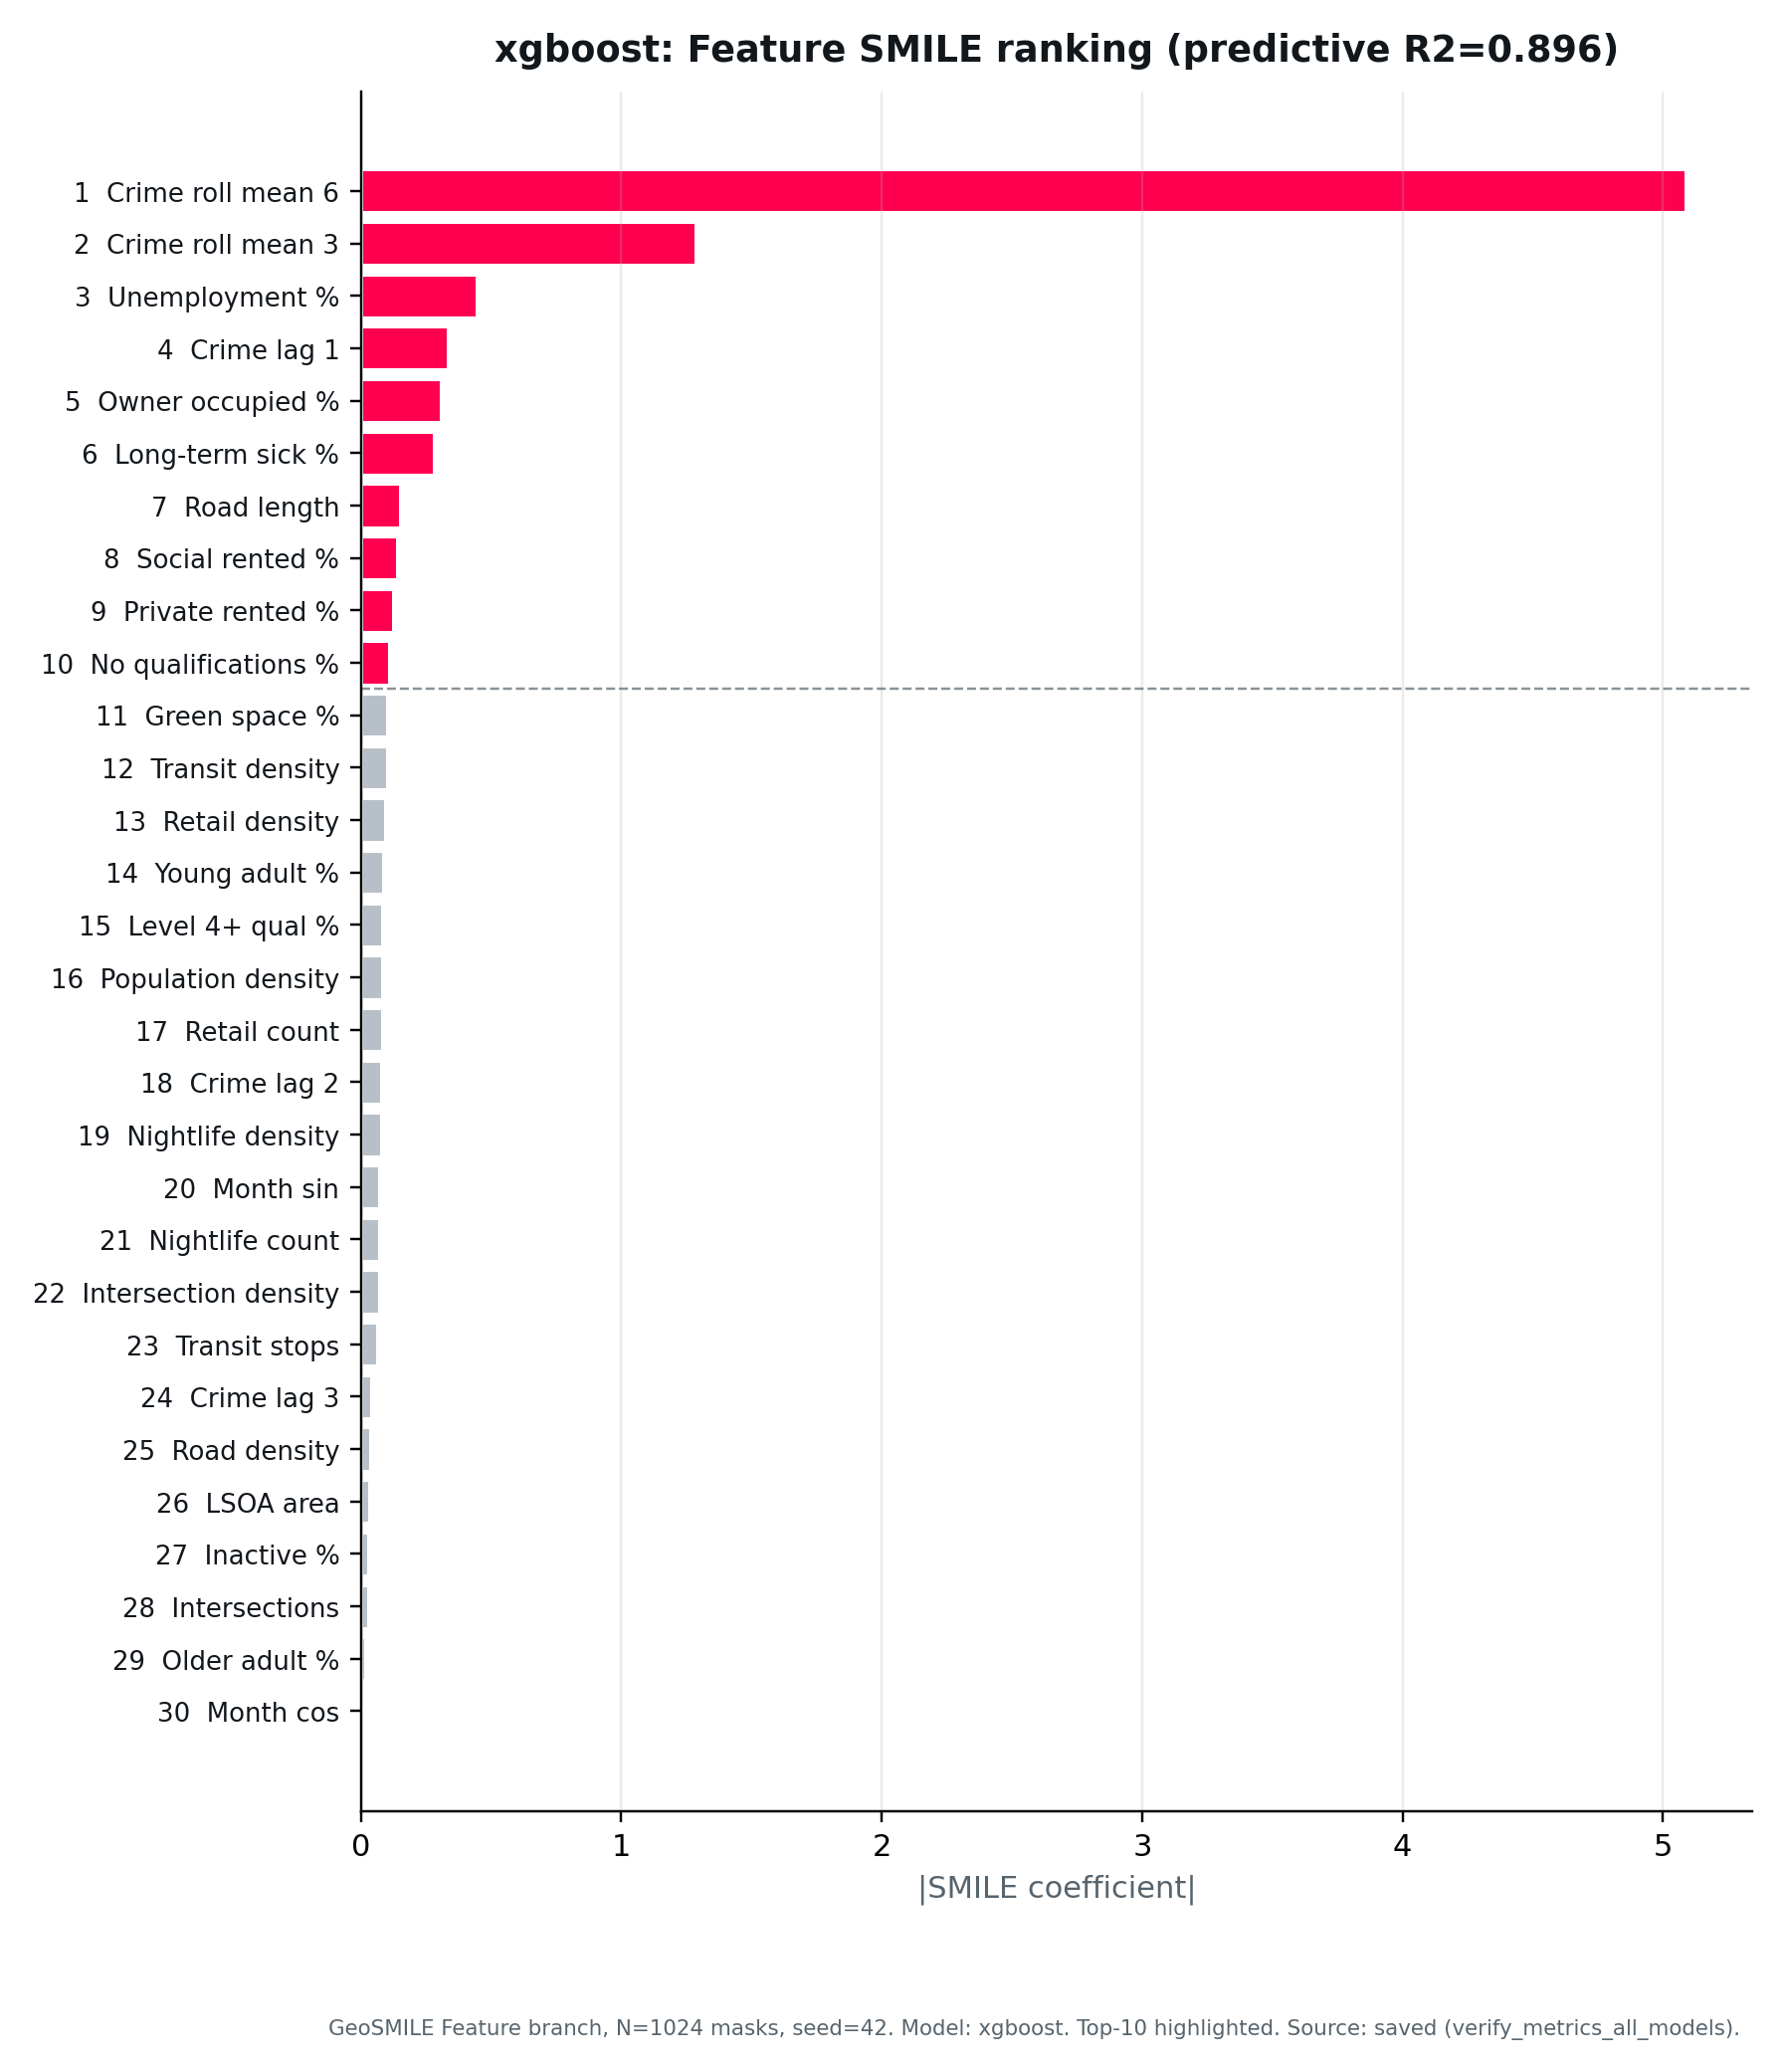
\includegraphics[width=\textwidth]{feature_top10_xgboost.png}
    \subcaption{XGBoost$^{\dagger}$}
    \label{fig:sel_feature_xgboost}
  \end{subfigure} \hfill
  \begin{subfigure}[t]{0.23\textwidth}
    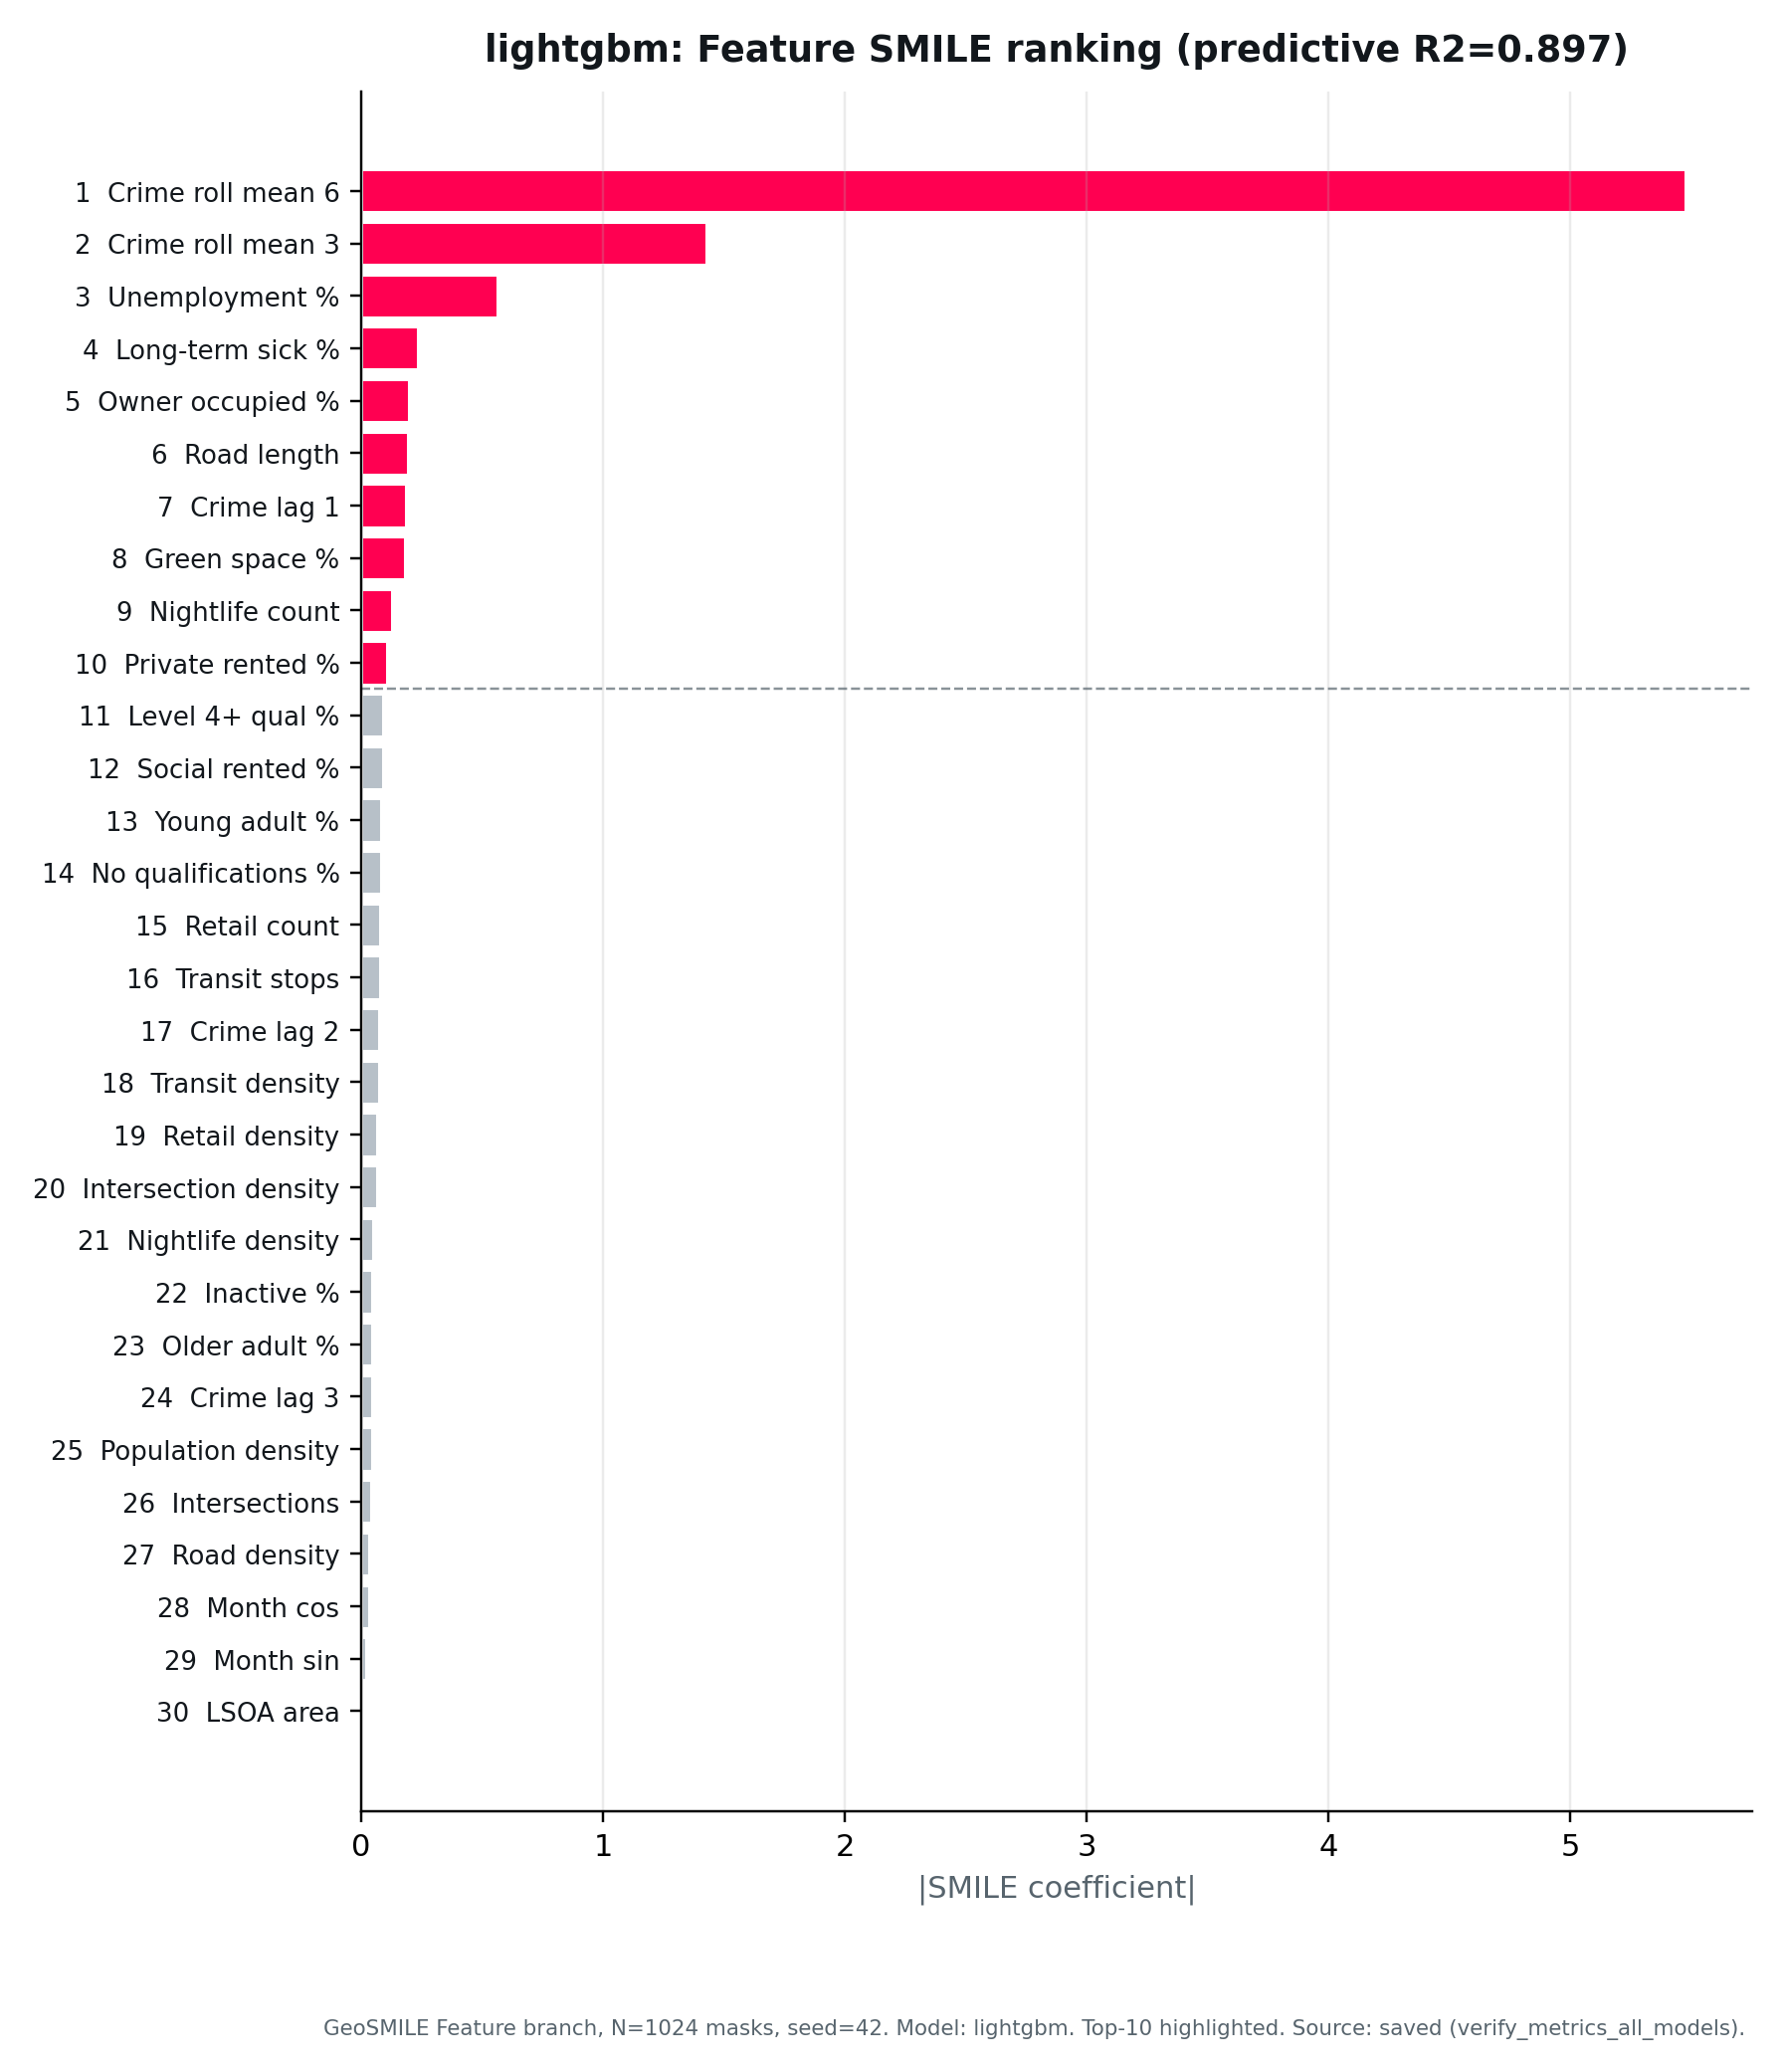
\includegraphics[width=\textwidth]{feature_top10_lightgbm.png}
    \subcaption{LightGBM$^{\dagger}$}
    \label{fig:sel_feature_lightgbm}
  \end{subfigure} \hfill
  \begin{subfigure}[t]{0.23\textwidth}
    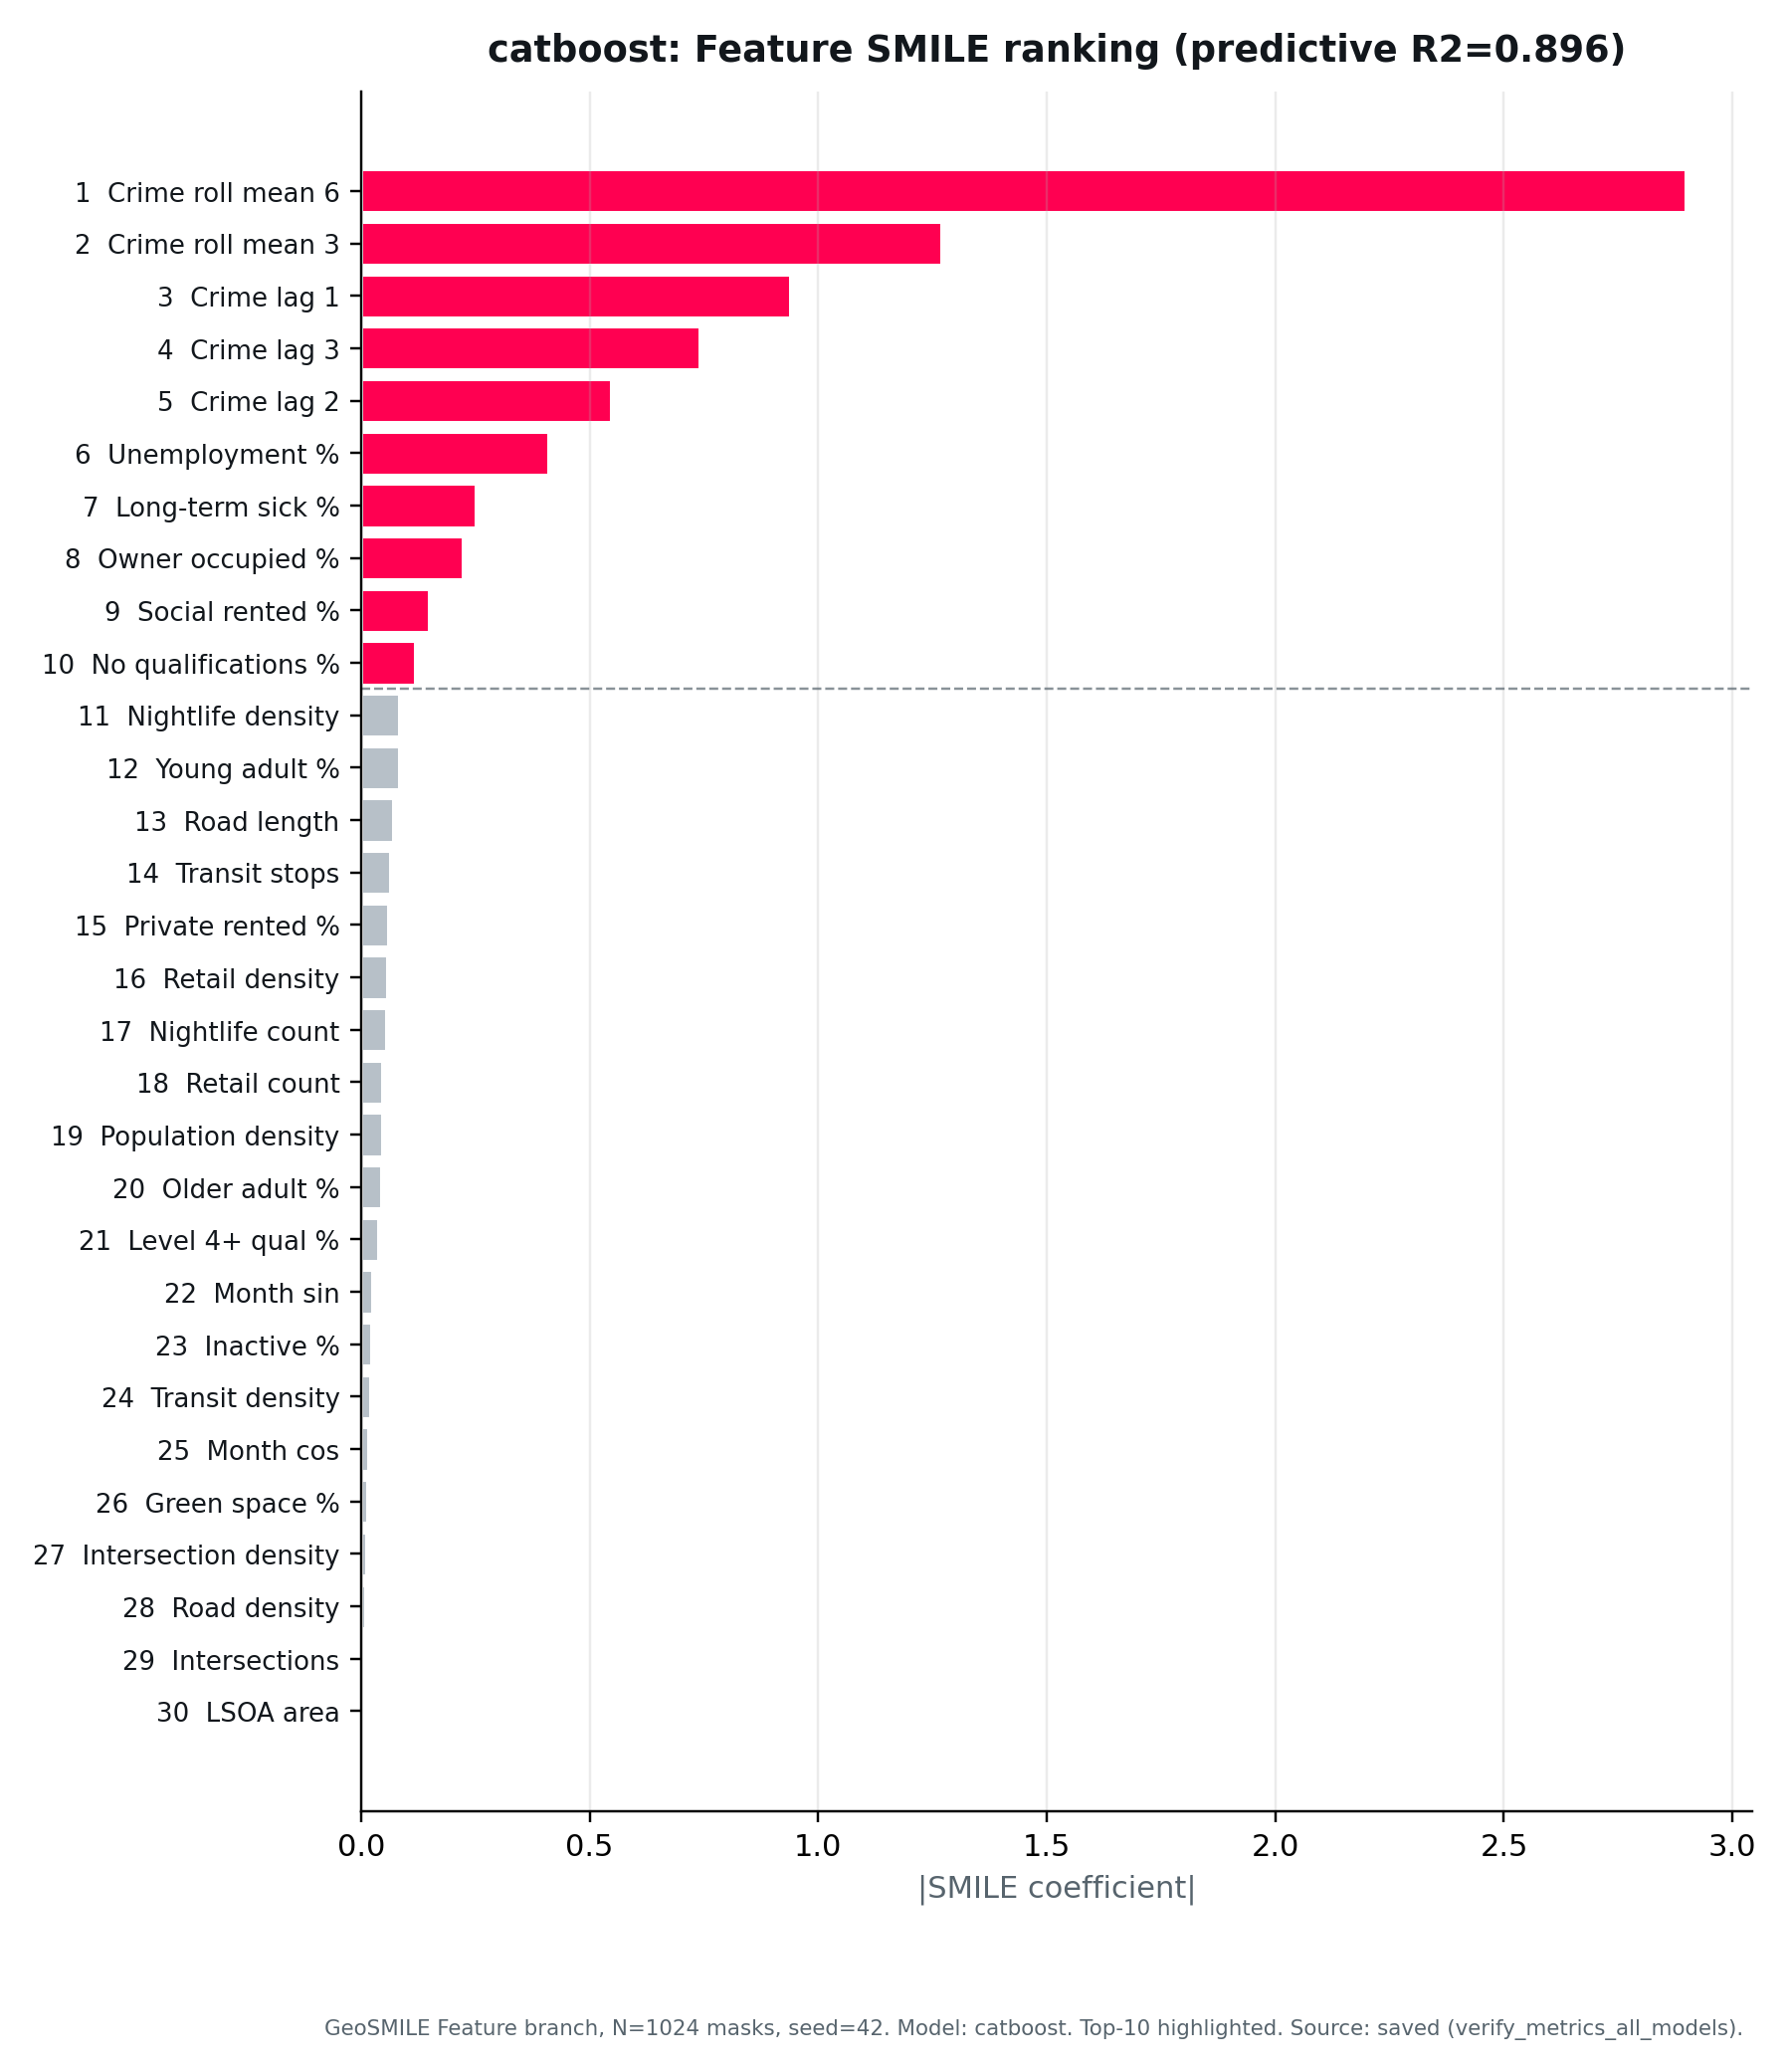
\includegraphics[width=\textwidth]{feature_top10_catboost.png}
    \subcaption{CatBoost$^{\dagger}$}
    \label{fig:sel_feature_catboost}
  \end{subfigure} \hfill
  \begin{subfigure}[t]{0.23\textwidth}
    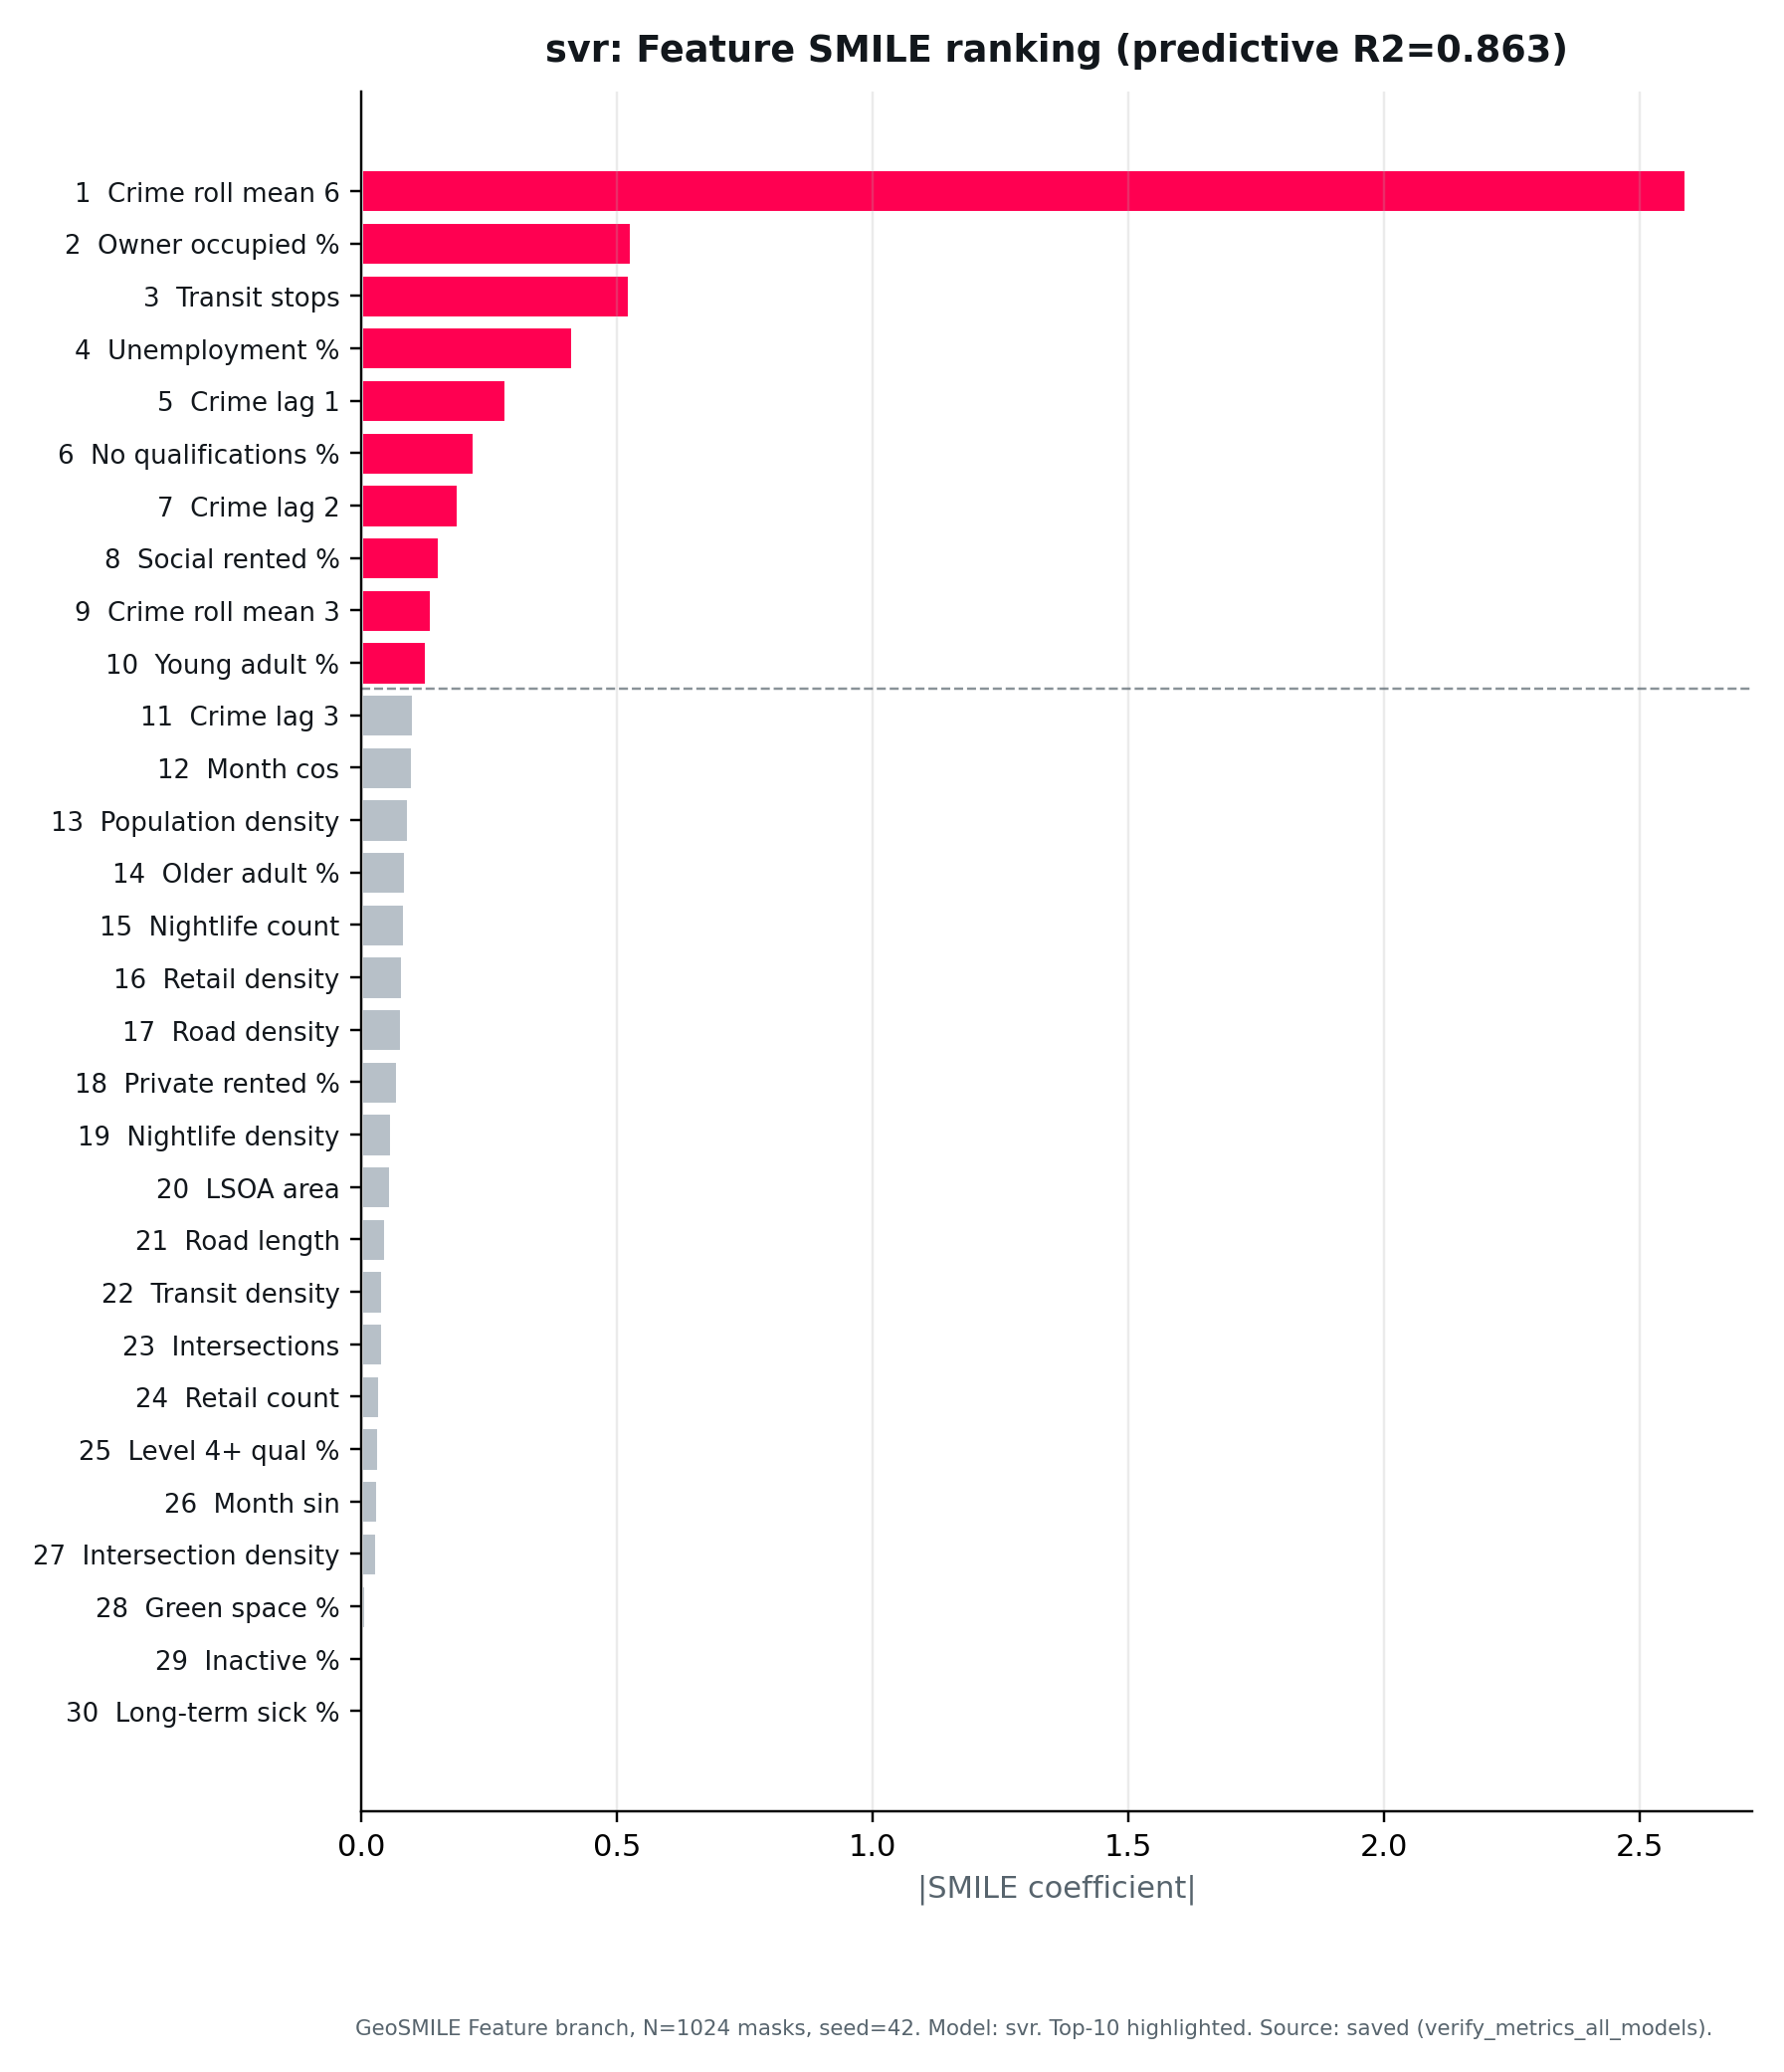
\includegraphics[width=\textwidth]{feature_top10_svr.png}
    \subcaption{SVR$^{\dagger}$}
    \label{fig:sel_feature_svr}
  \end{subfigure}

  \vspace{0.6em}

  \begin{subfigure}[t]{0.23\textwidth}
    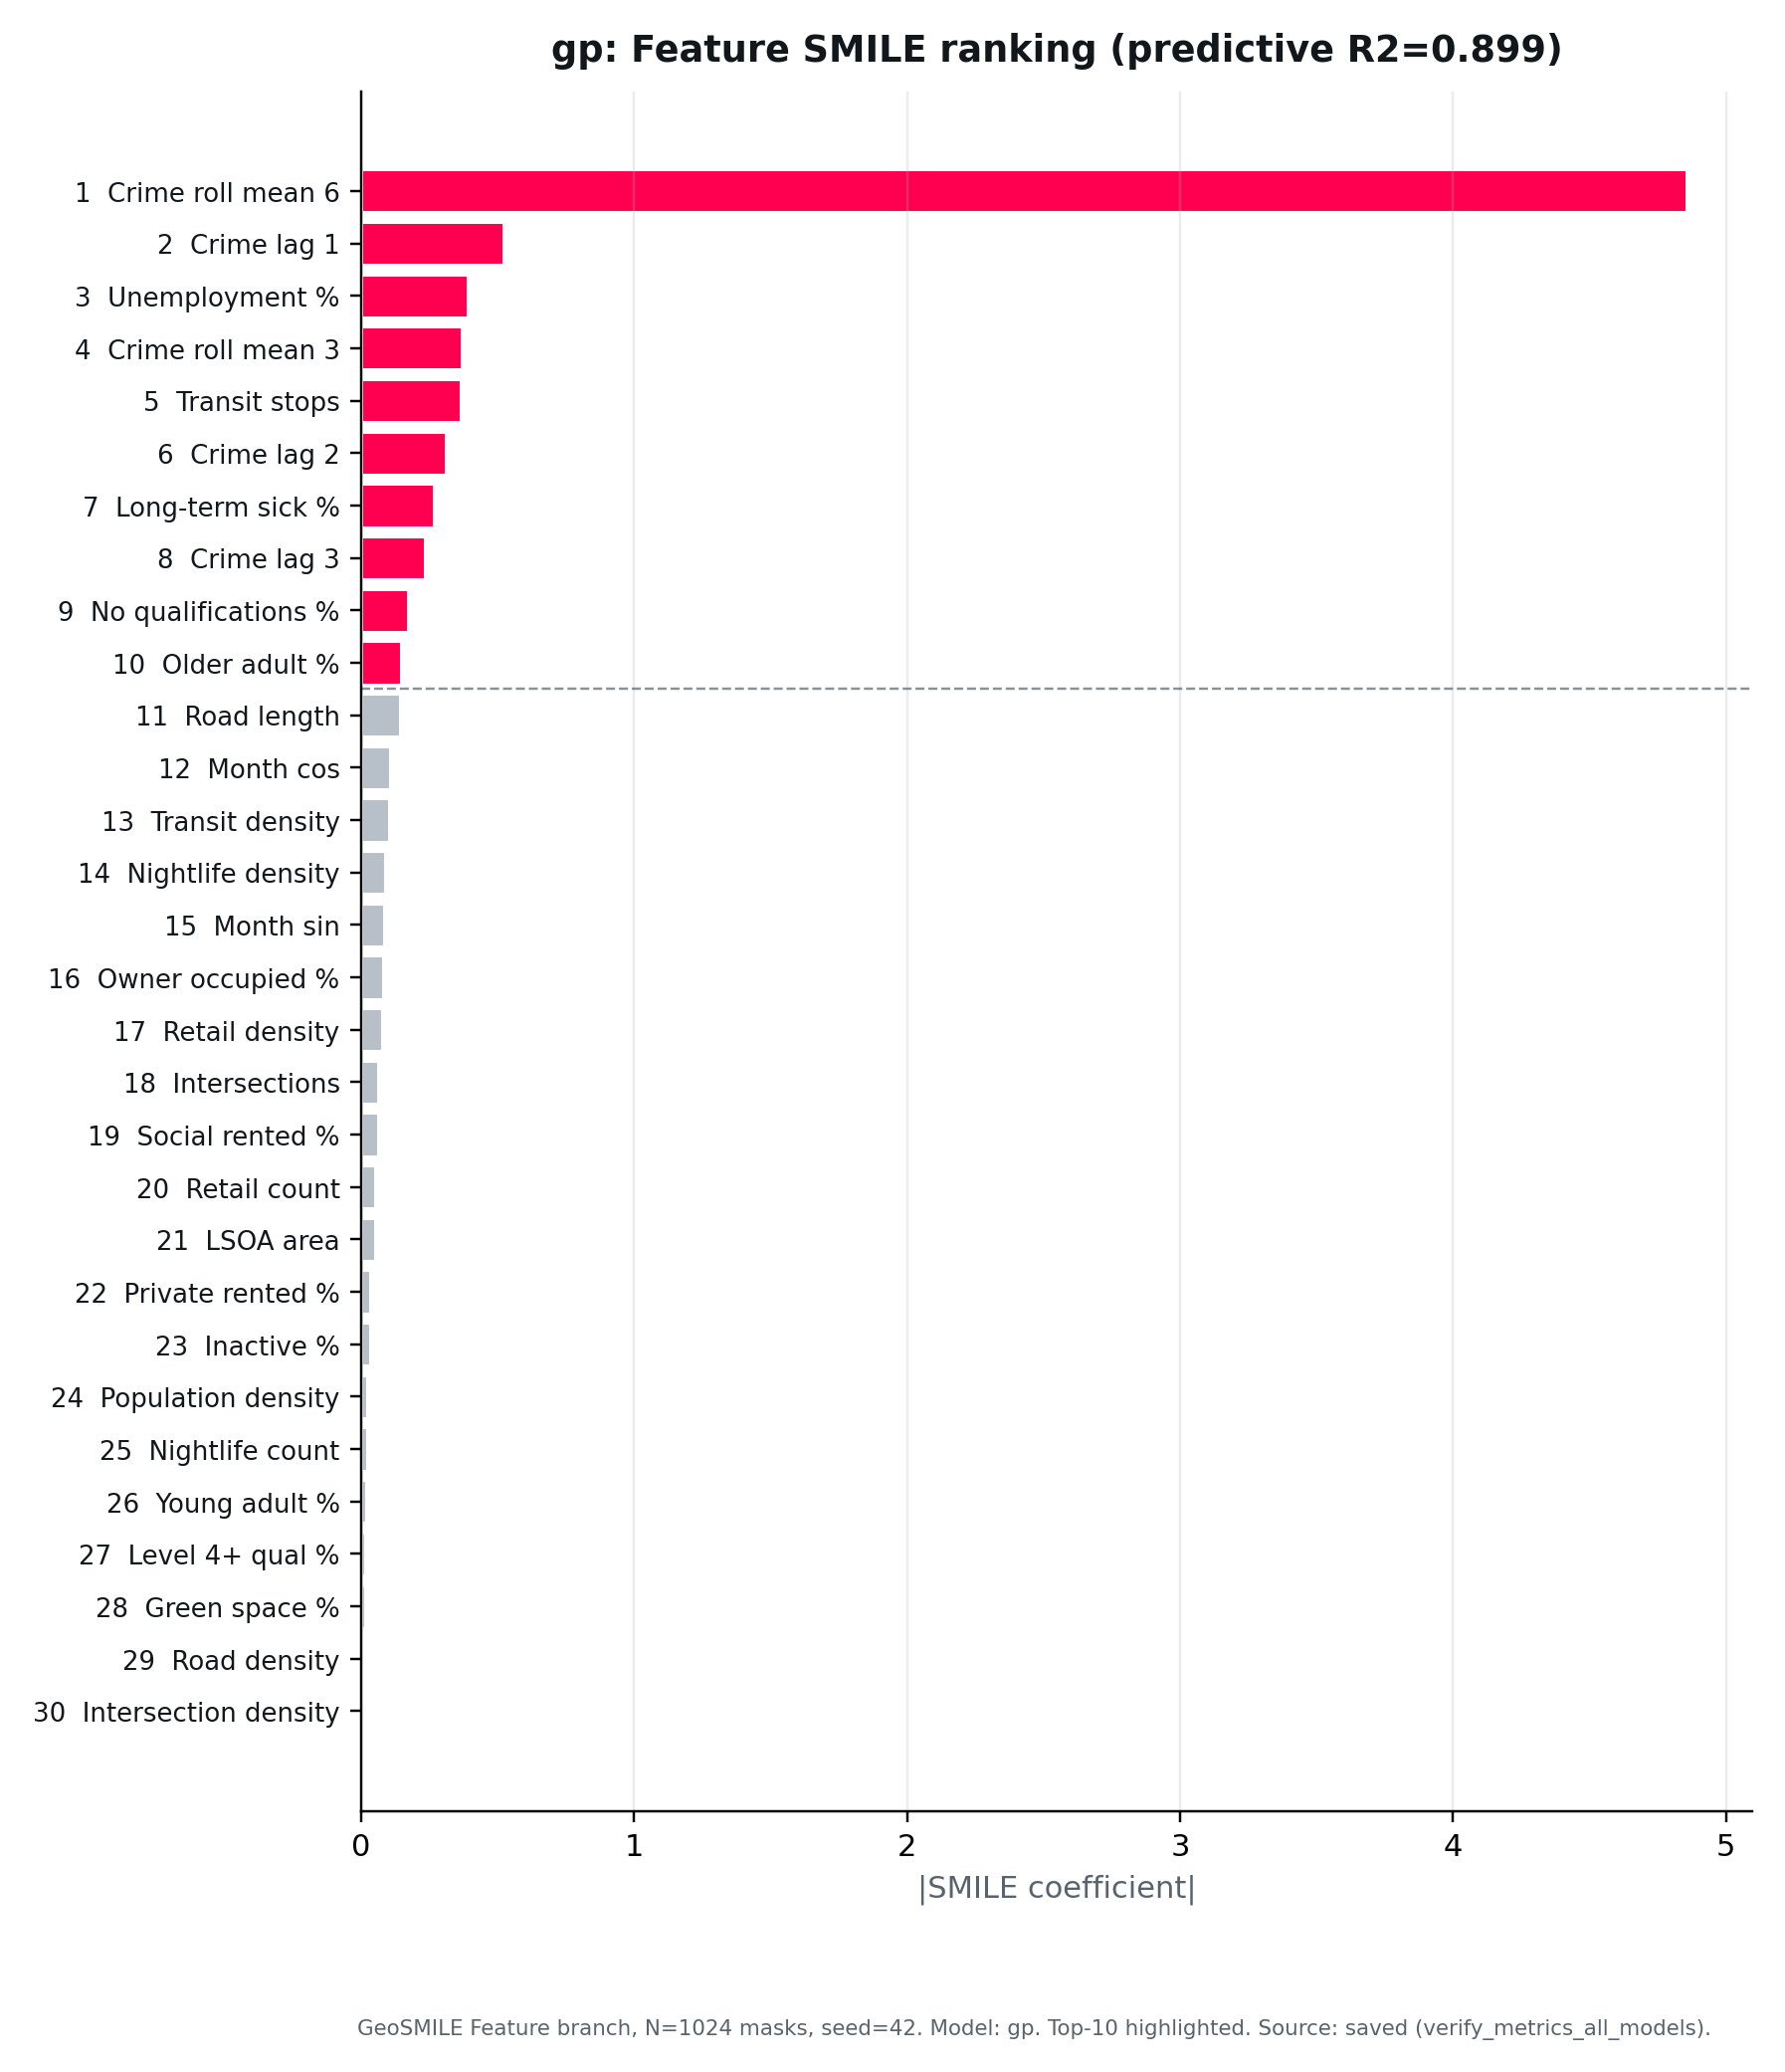
\includegraphics[width=\textwidth]{feature_top10_gp.png}
    \subcaption{GP$^{\dagger}$}
    \label{fig:sel_feature_gp}
  \end{subfigure} \hfill
  \begin{subfigure}[t]{0.23\textwidth}
    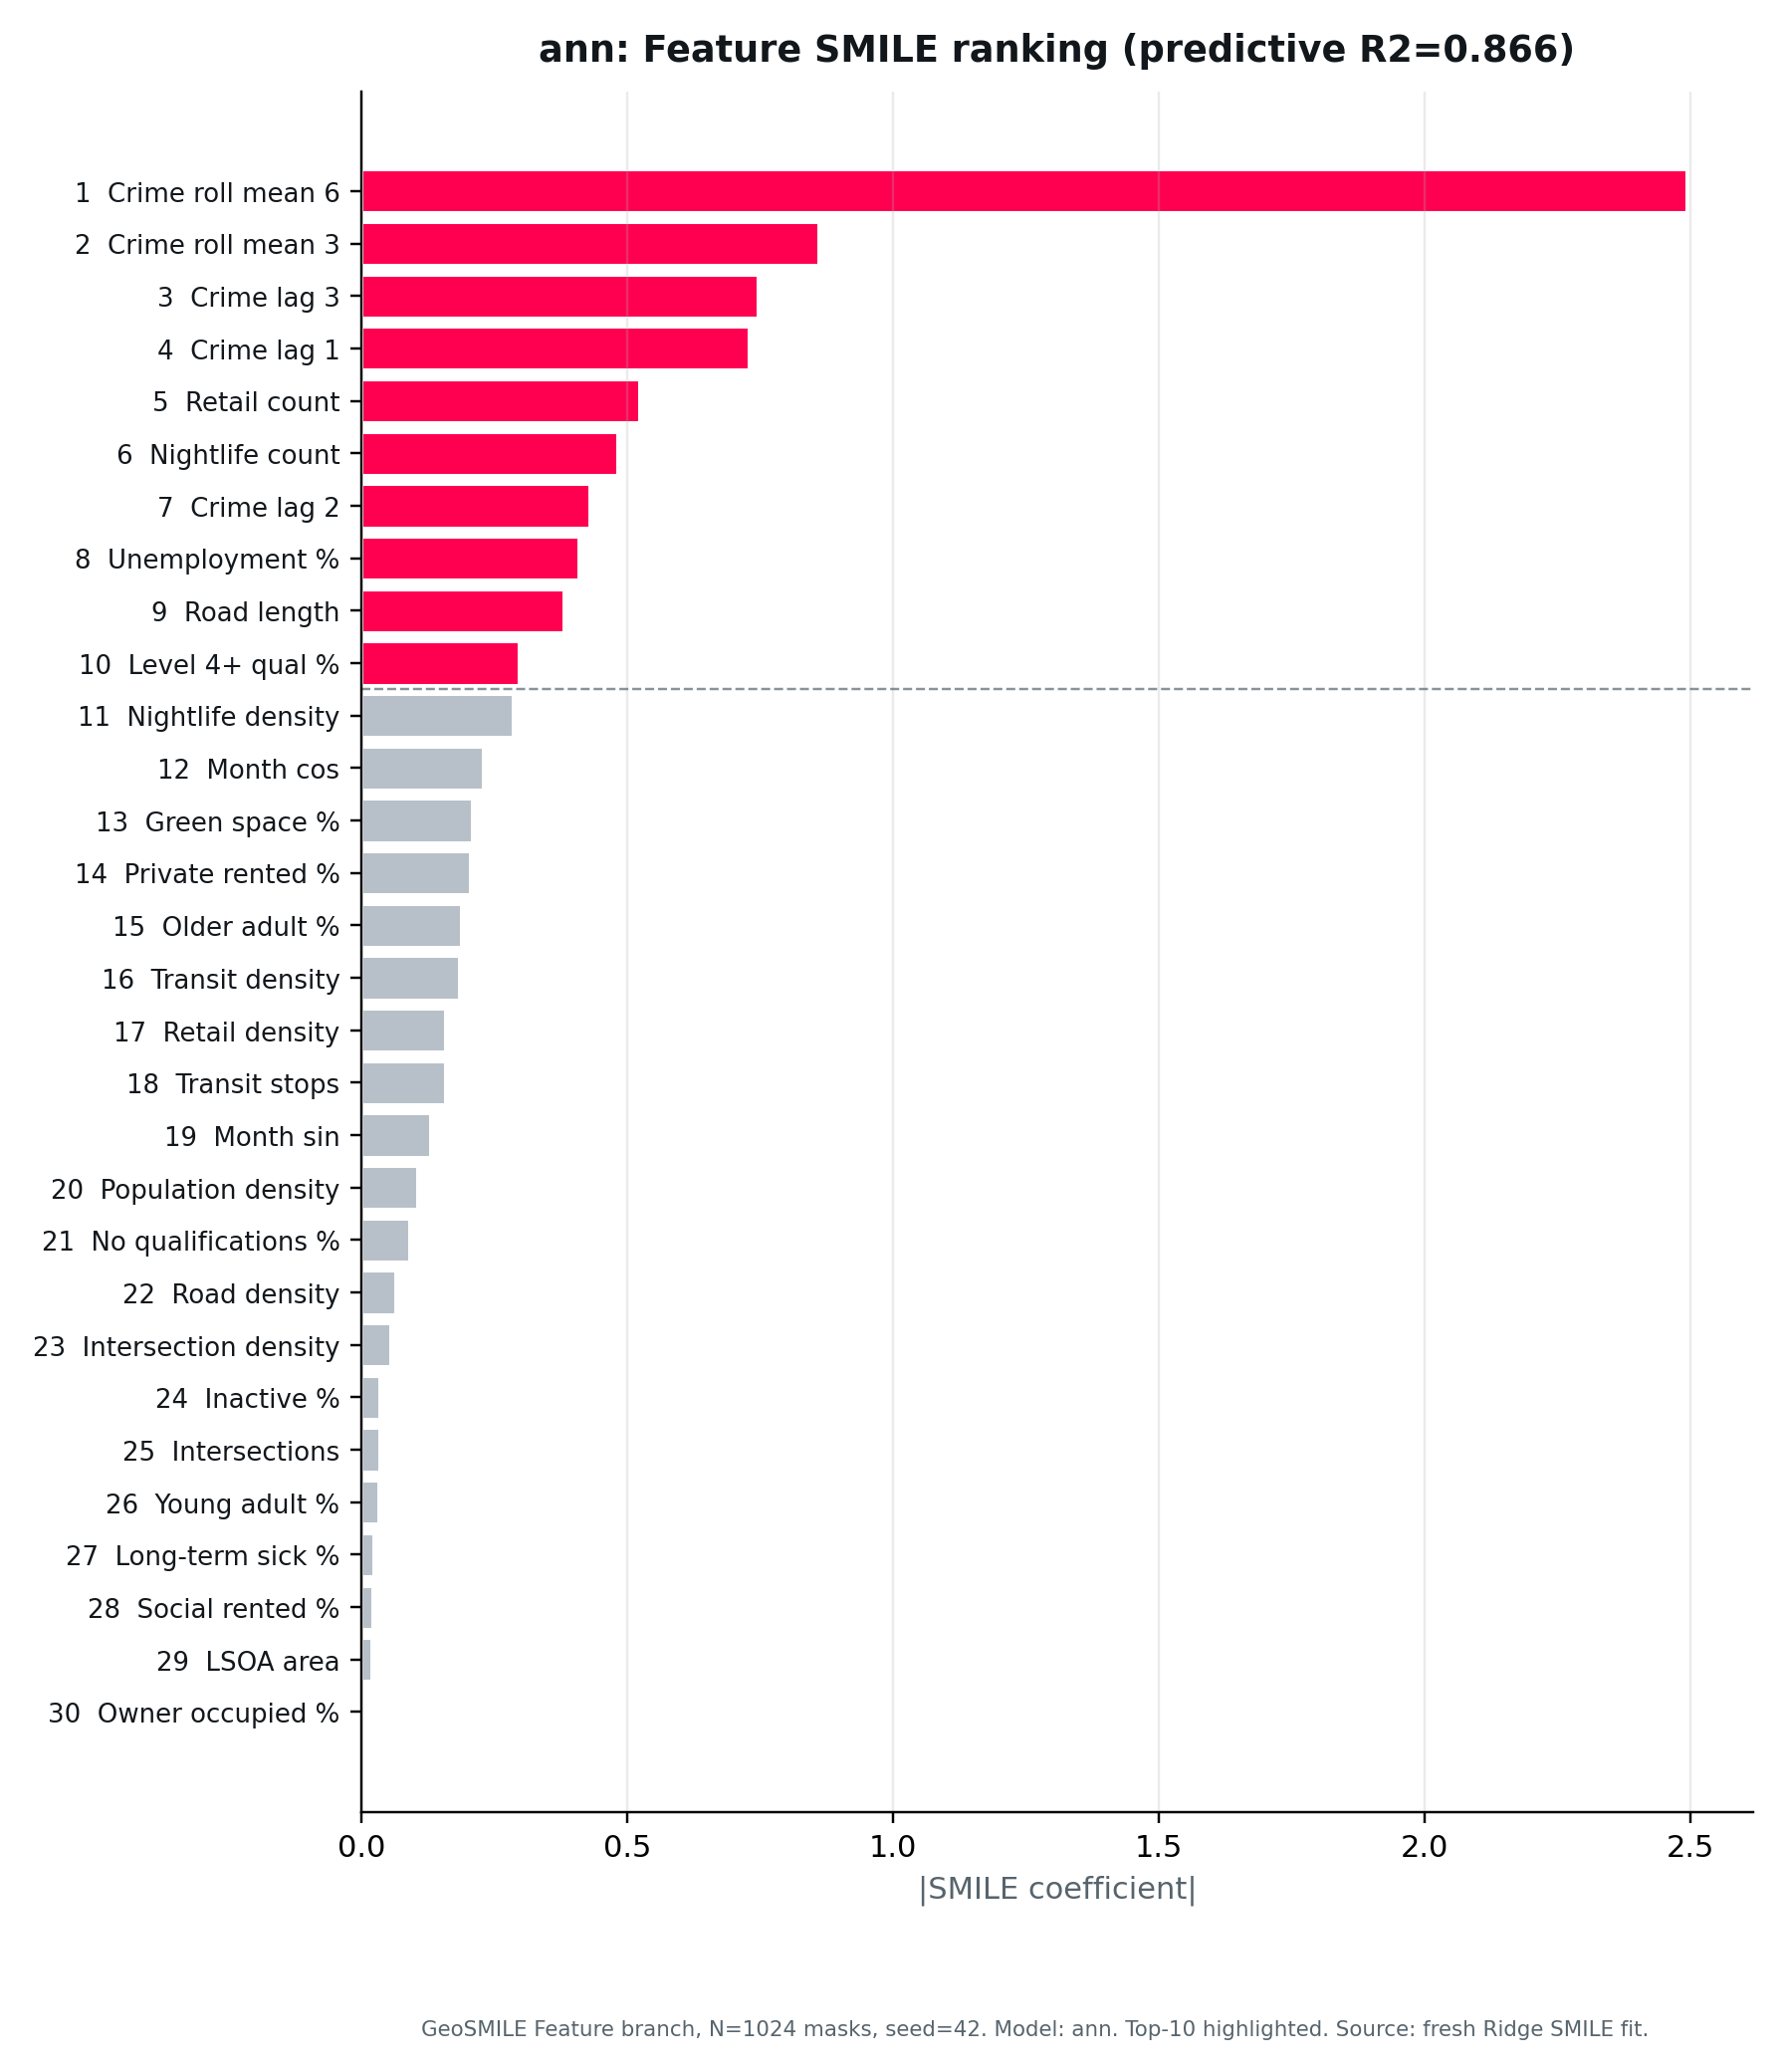
\includegraphics[width=\textwidth]{feature_top10_ann.png}
    \subcaption{ANN$^{\ddagger}$}
    \label{fig:sel_feature_ann}
  \end{subfigure} \hfill
  \begin{subfigure}[t]{0.23\textwidth}
    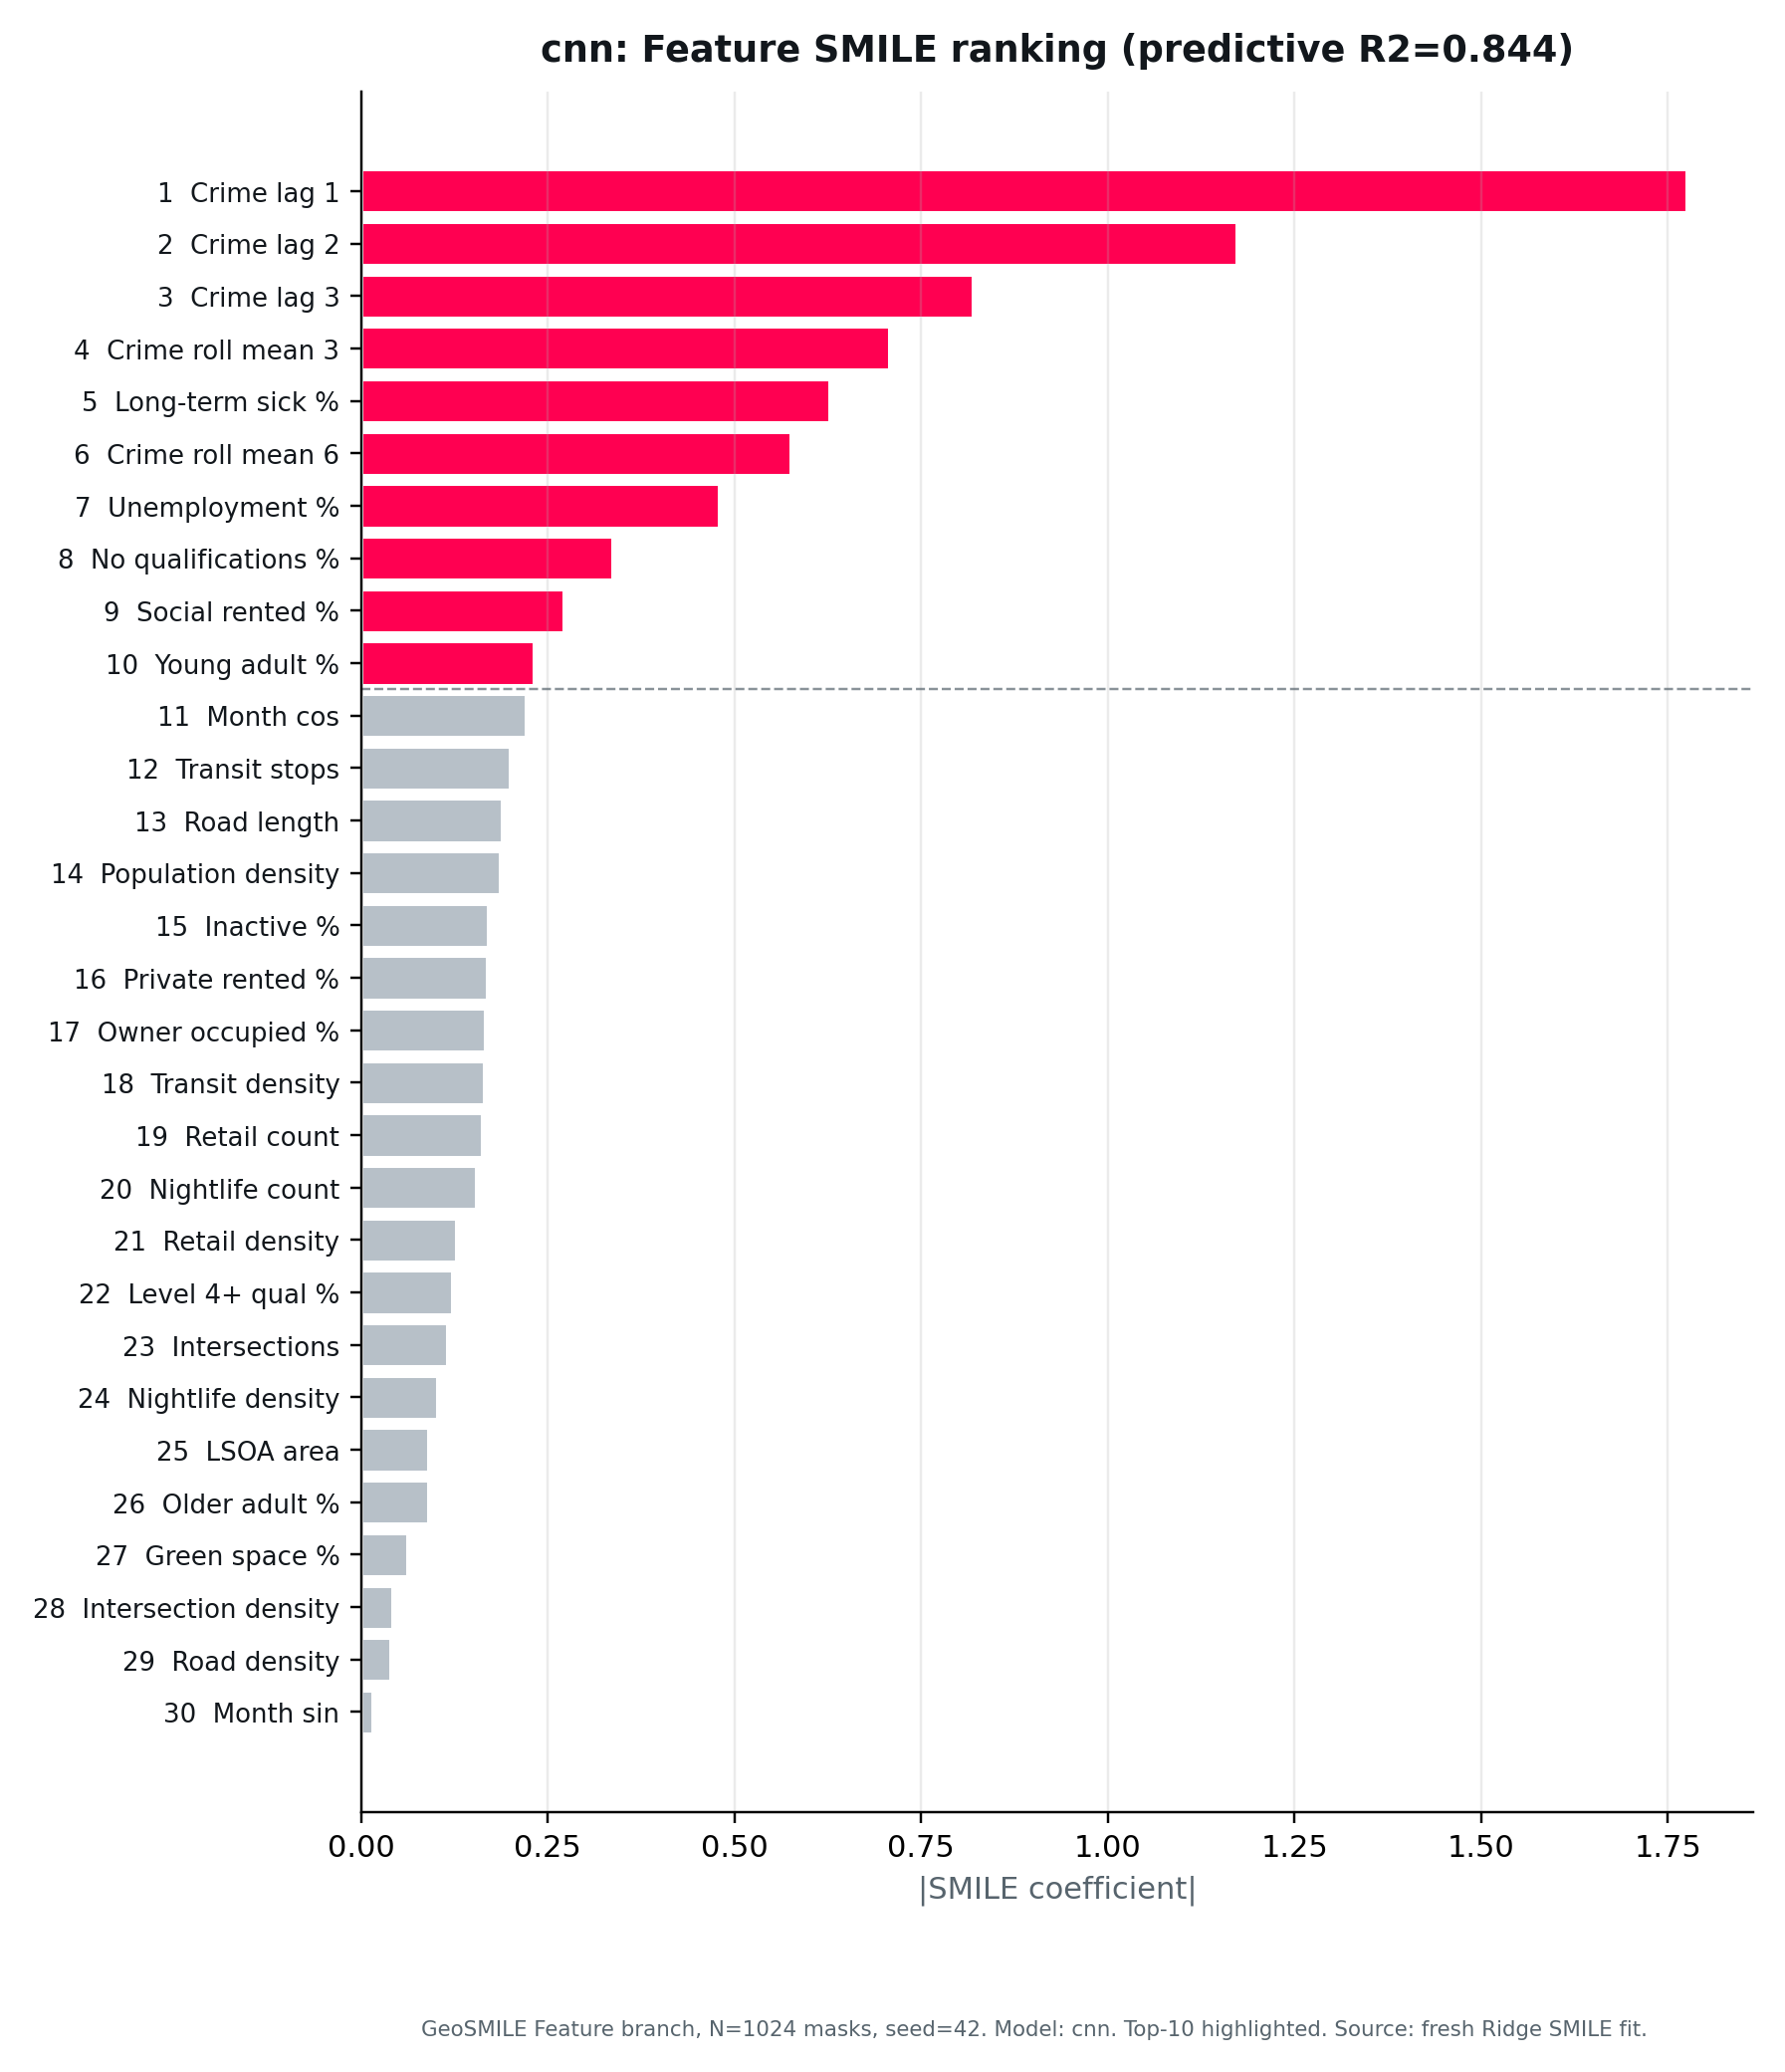
\includegraphics[width=\textwidth]{feature_top10_cnn.png}
    \subcaption{CNN$^{\ddagger}$}
    \label{fig:sel_feature_cnn}
  \end{subfigure} \hfill
  \begin{subfigure}[t]{0.23\textwidth}
    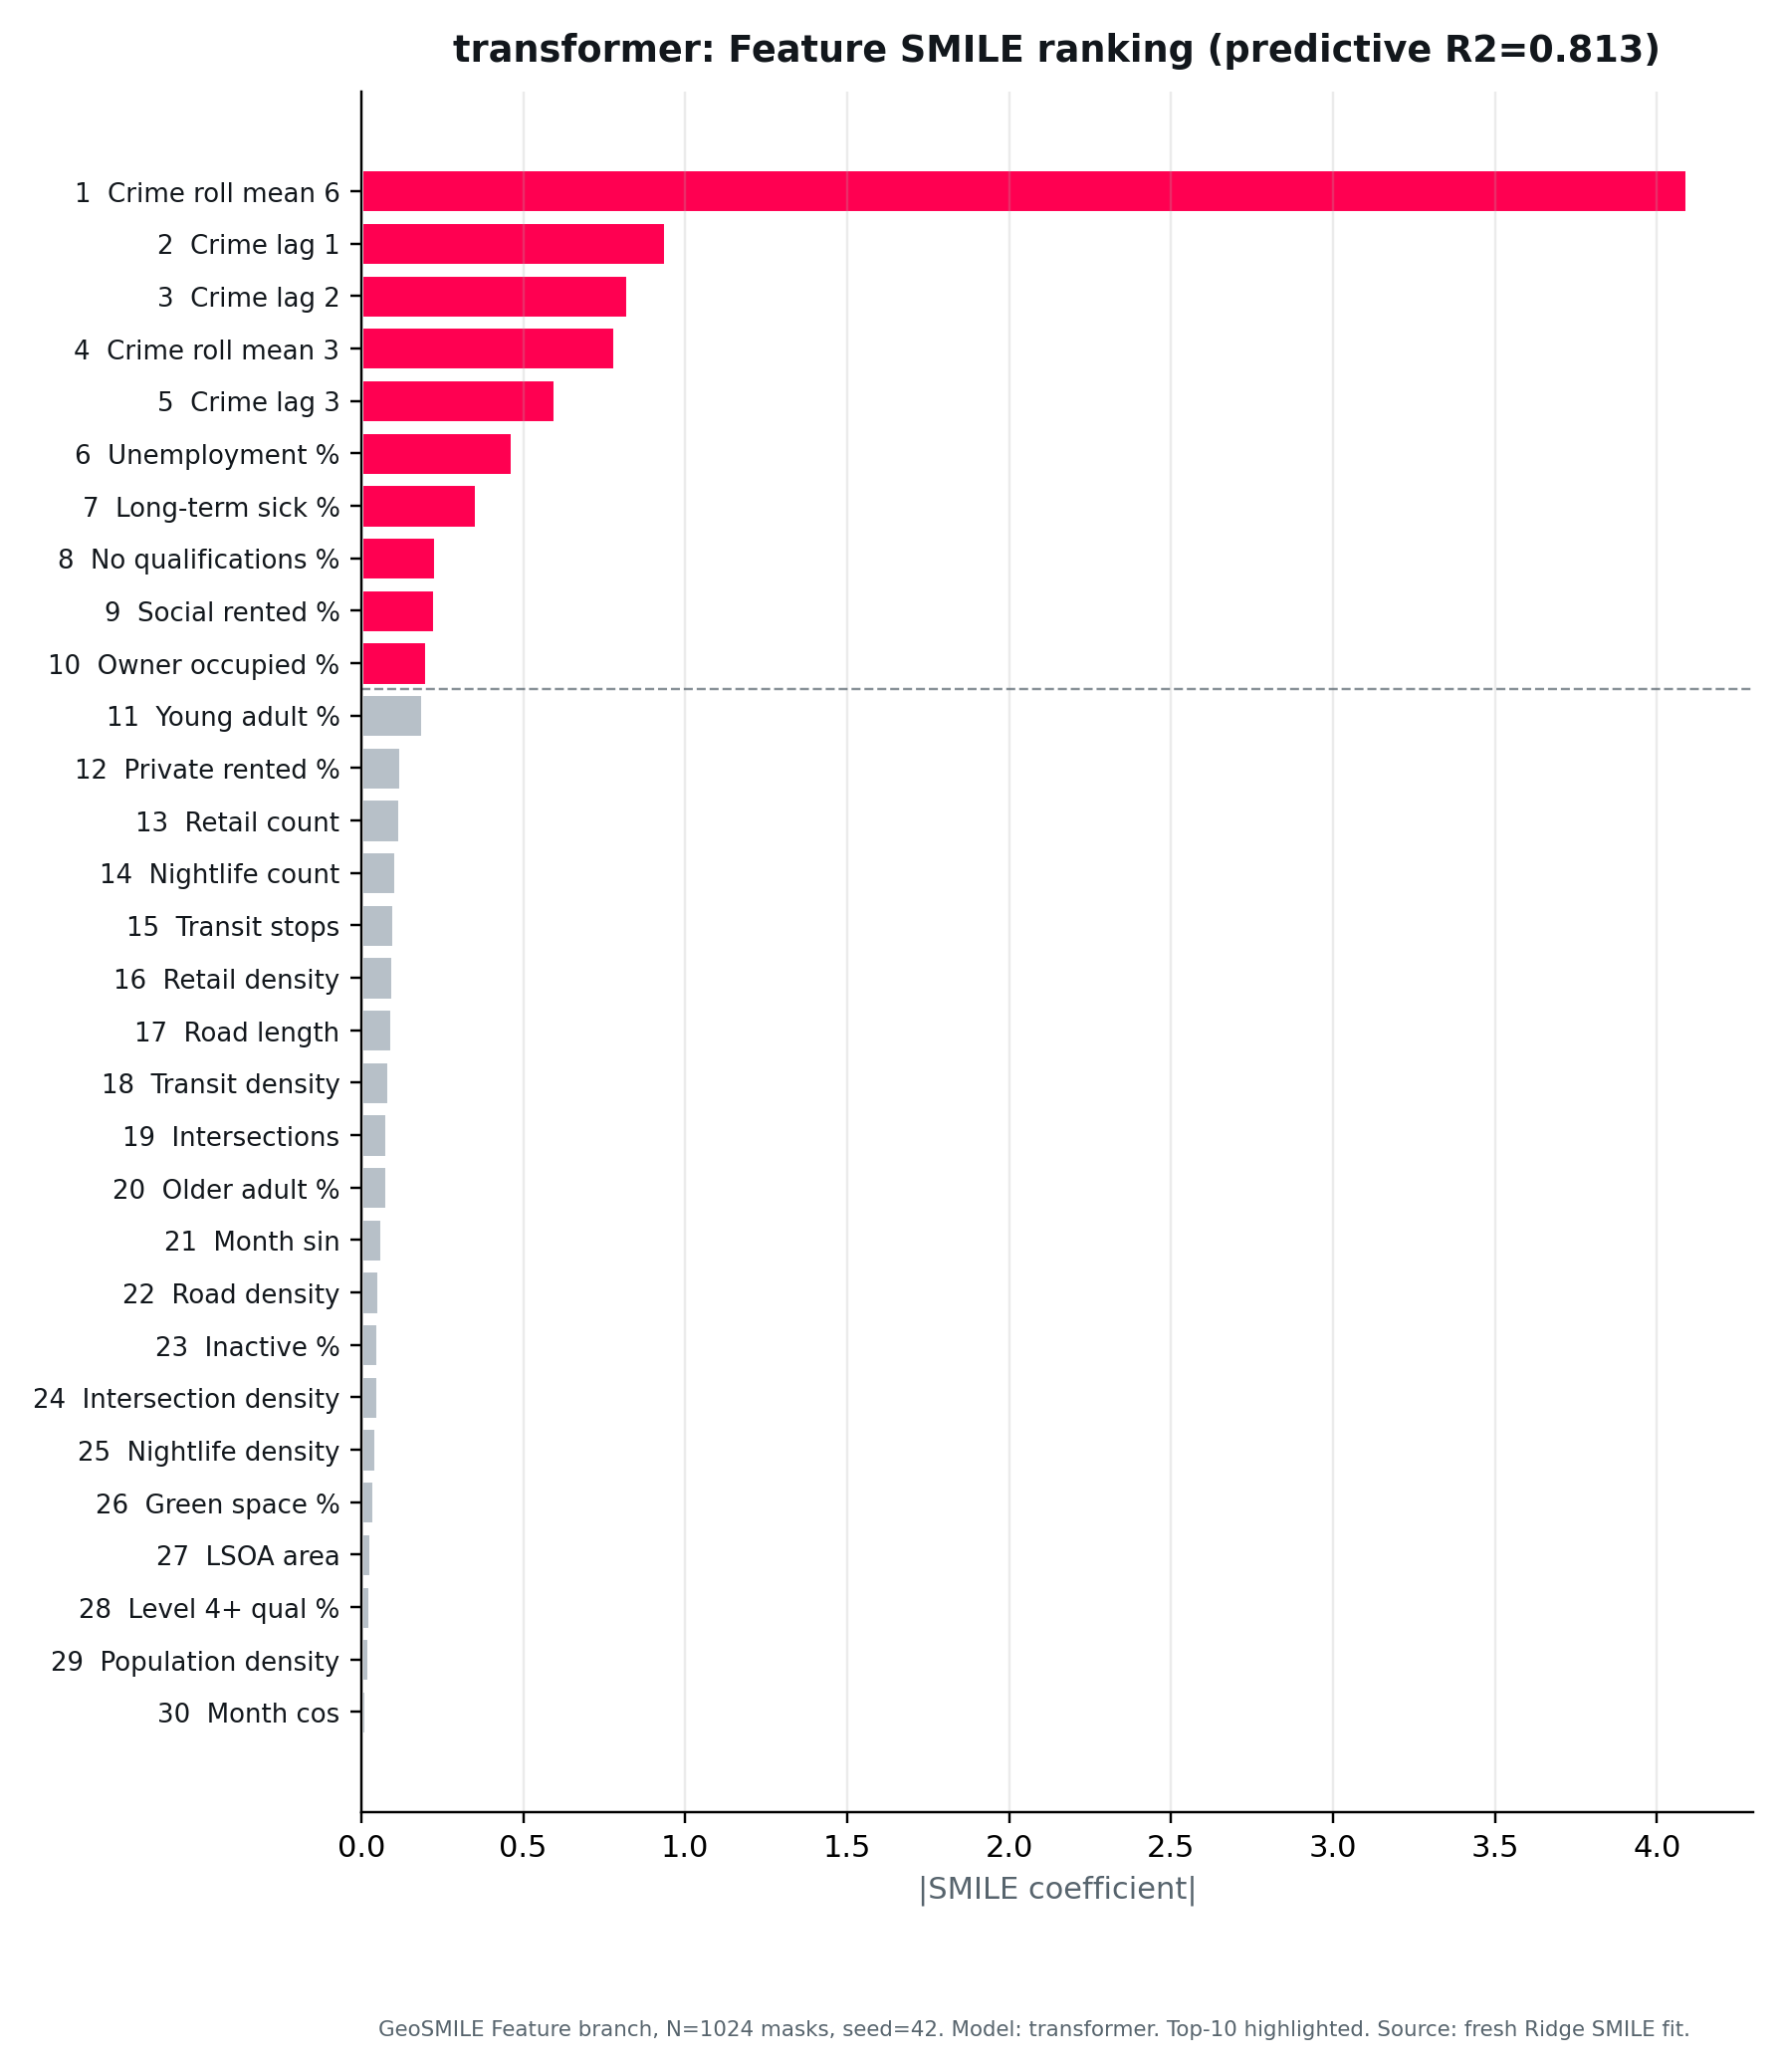
\includegraphics[width=\textwidth]{feature_top10_transformer.png}
    \subcaption{Transformer$^{\ddagger}$}
    \label{fig:sel_feature_transformer}
  \end{subfigure}
\caption{Feature SMILE top-10 ranking by candidate model, kernel-weighted
Ridge surrogate ($N{=}1{,}024$ masks, seed 42). Title reports each
model's held-out \emph{predictive} $R^2$ (not fidelity -- contrast
Figure~\ref{fig:sel_feature_rf}, whose two panels report fidelity
$R^2$ instead, since that is the quantity their surrogate choice was
selected to fix). Superscripts mark provenance per
Table~\ref{tab:sel_provenance}: $\dagger$ saved from the rigorous
7-model verification (full metric suite); $\ddagger$ a fresh Ridge SMILE
fit for this round of design experiments (fidelity-focused only).}
\label{fig:sel_feature_ridge}
\end{figure}

\begin{figure}[htbp]
\centering
  \begin{subfigure}[t]{0.32\textwidth}
    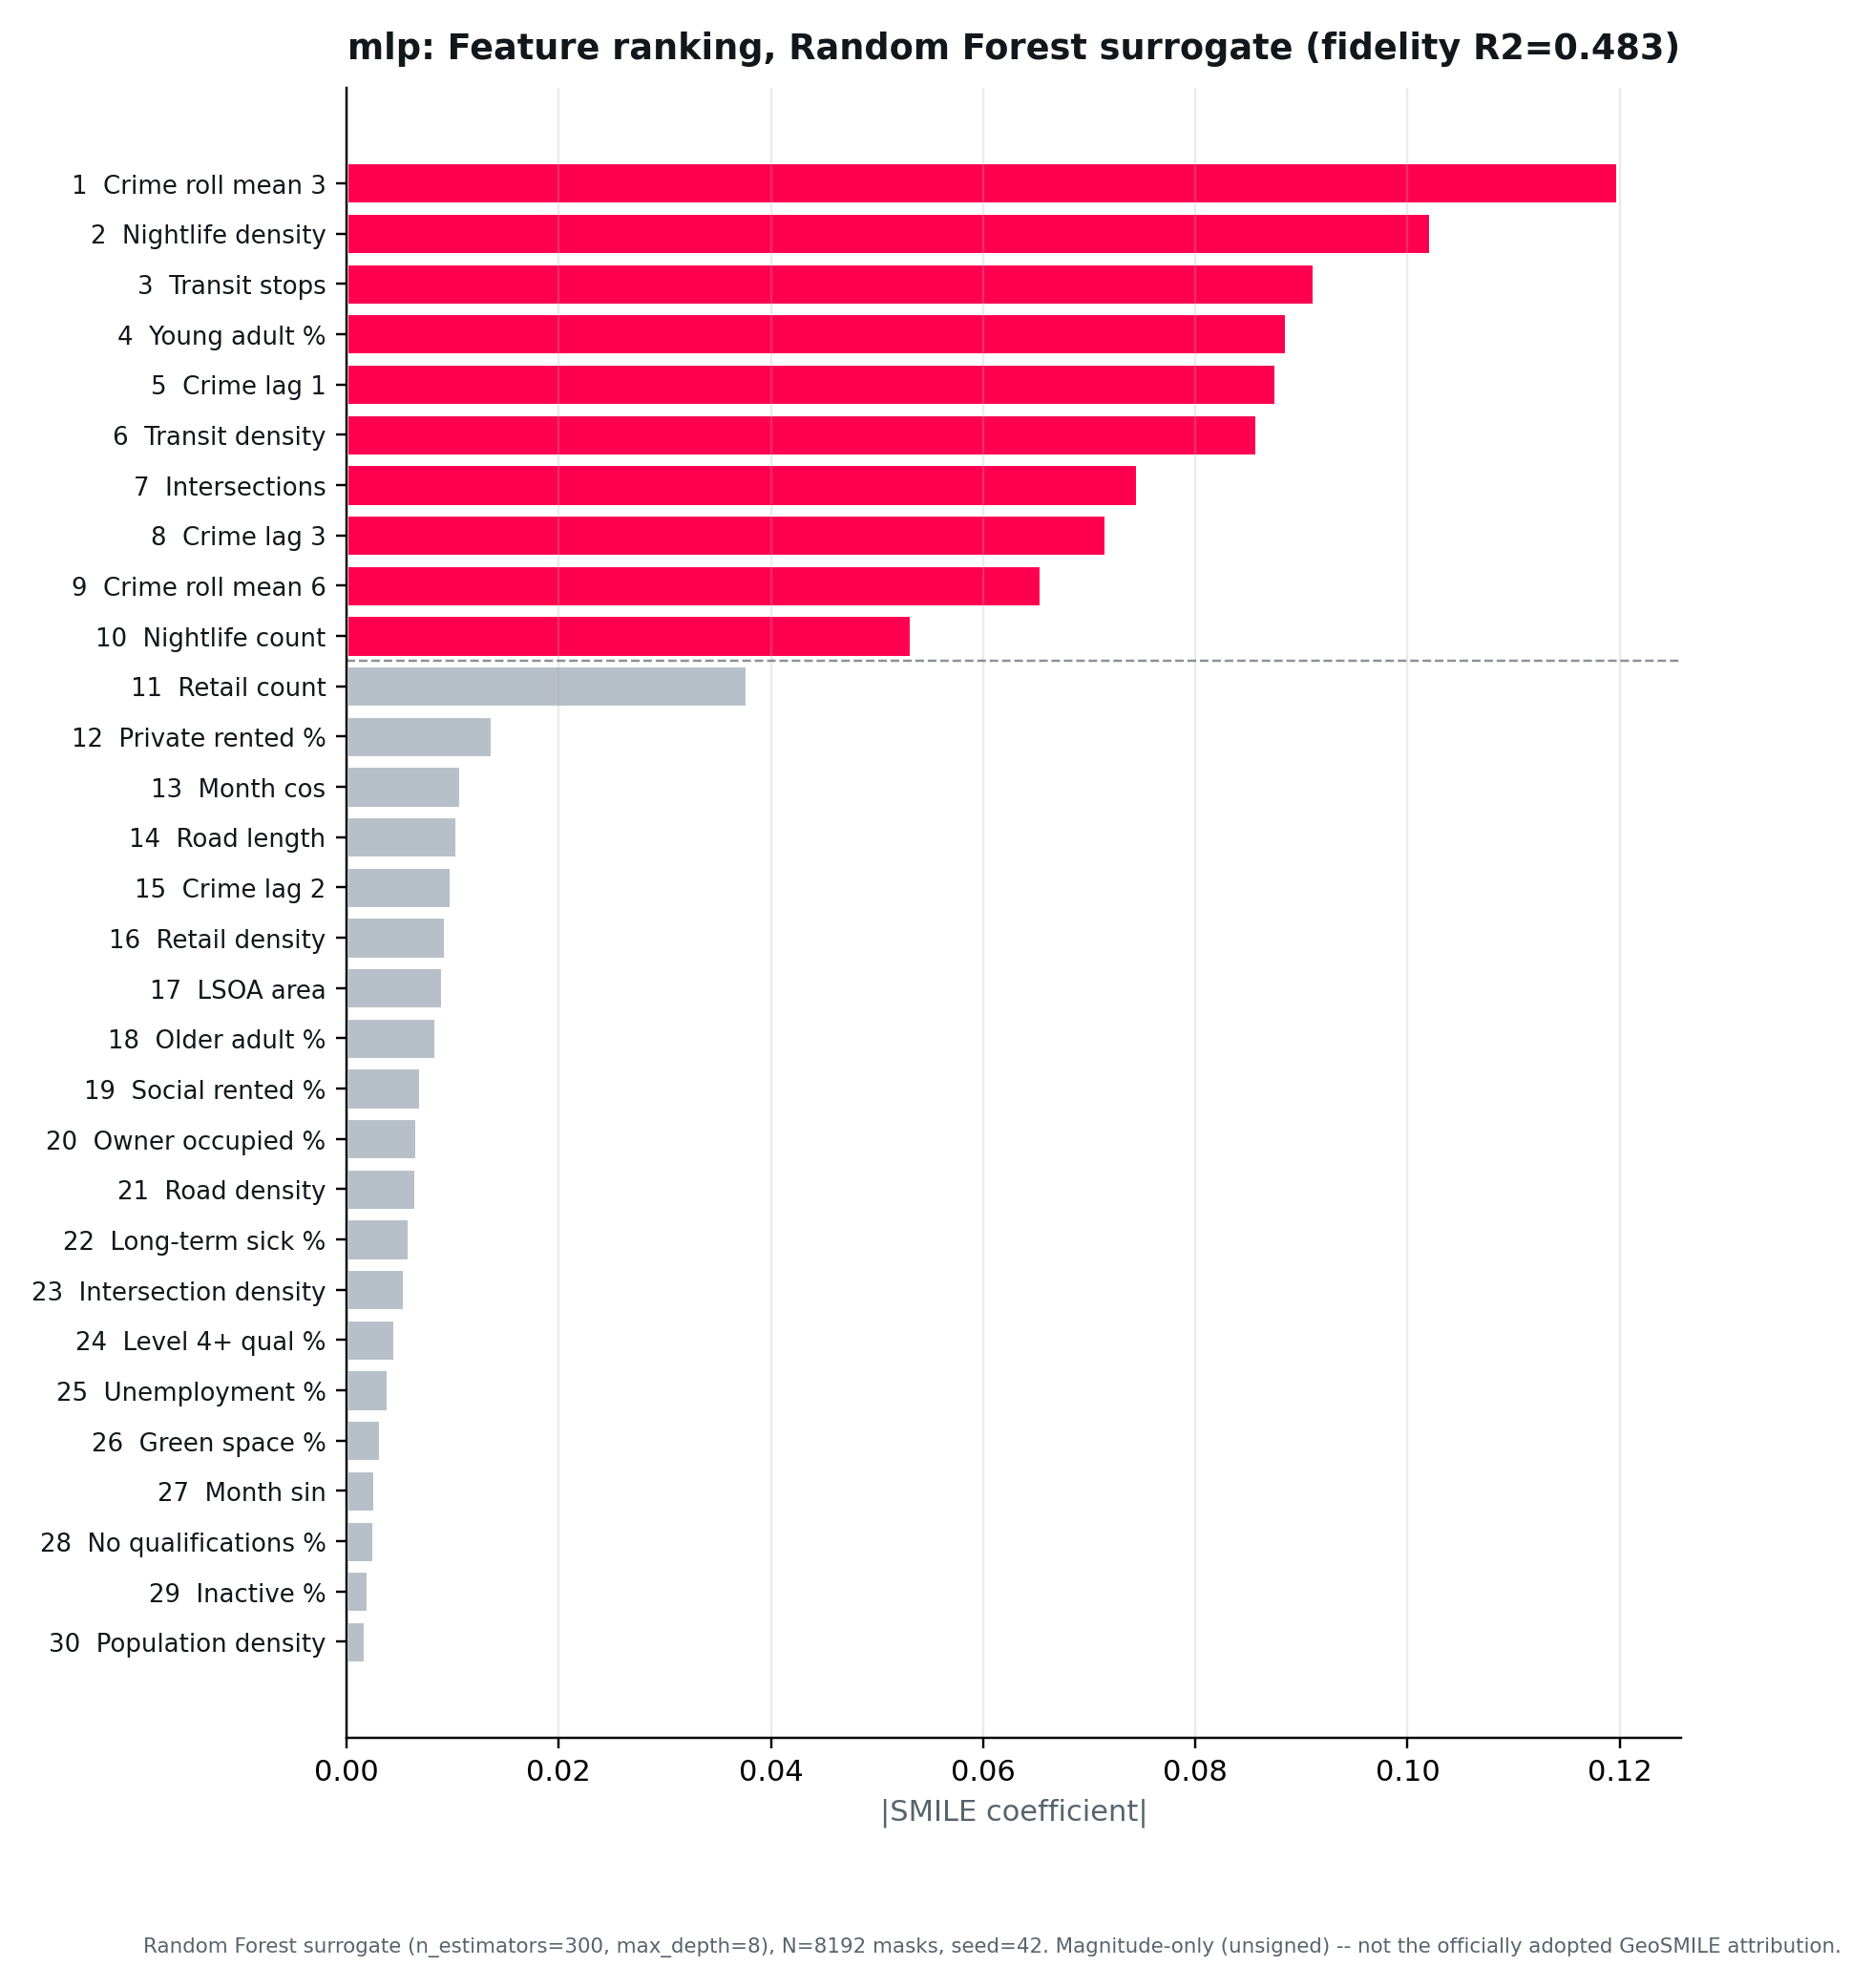
\includegraphics[width=\textwidth]{feature_top10_mlp.png}
    \subcaption{MLP (shallow)$^{\P}$ \\ {\scriptsize Random Forest, $N{=}8{,}192$, kernel-weighted}}
    \label{fig:sel_feature_mlp}
  \end{subfigure} \hfill
  \begin{subfigure}[t]{0.32\textwidth}
    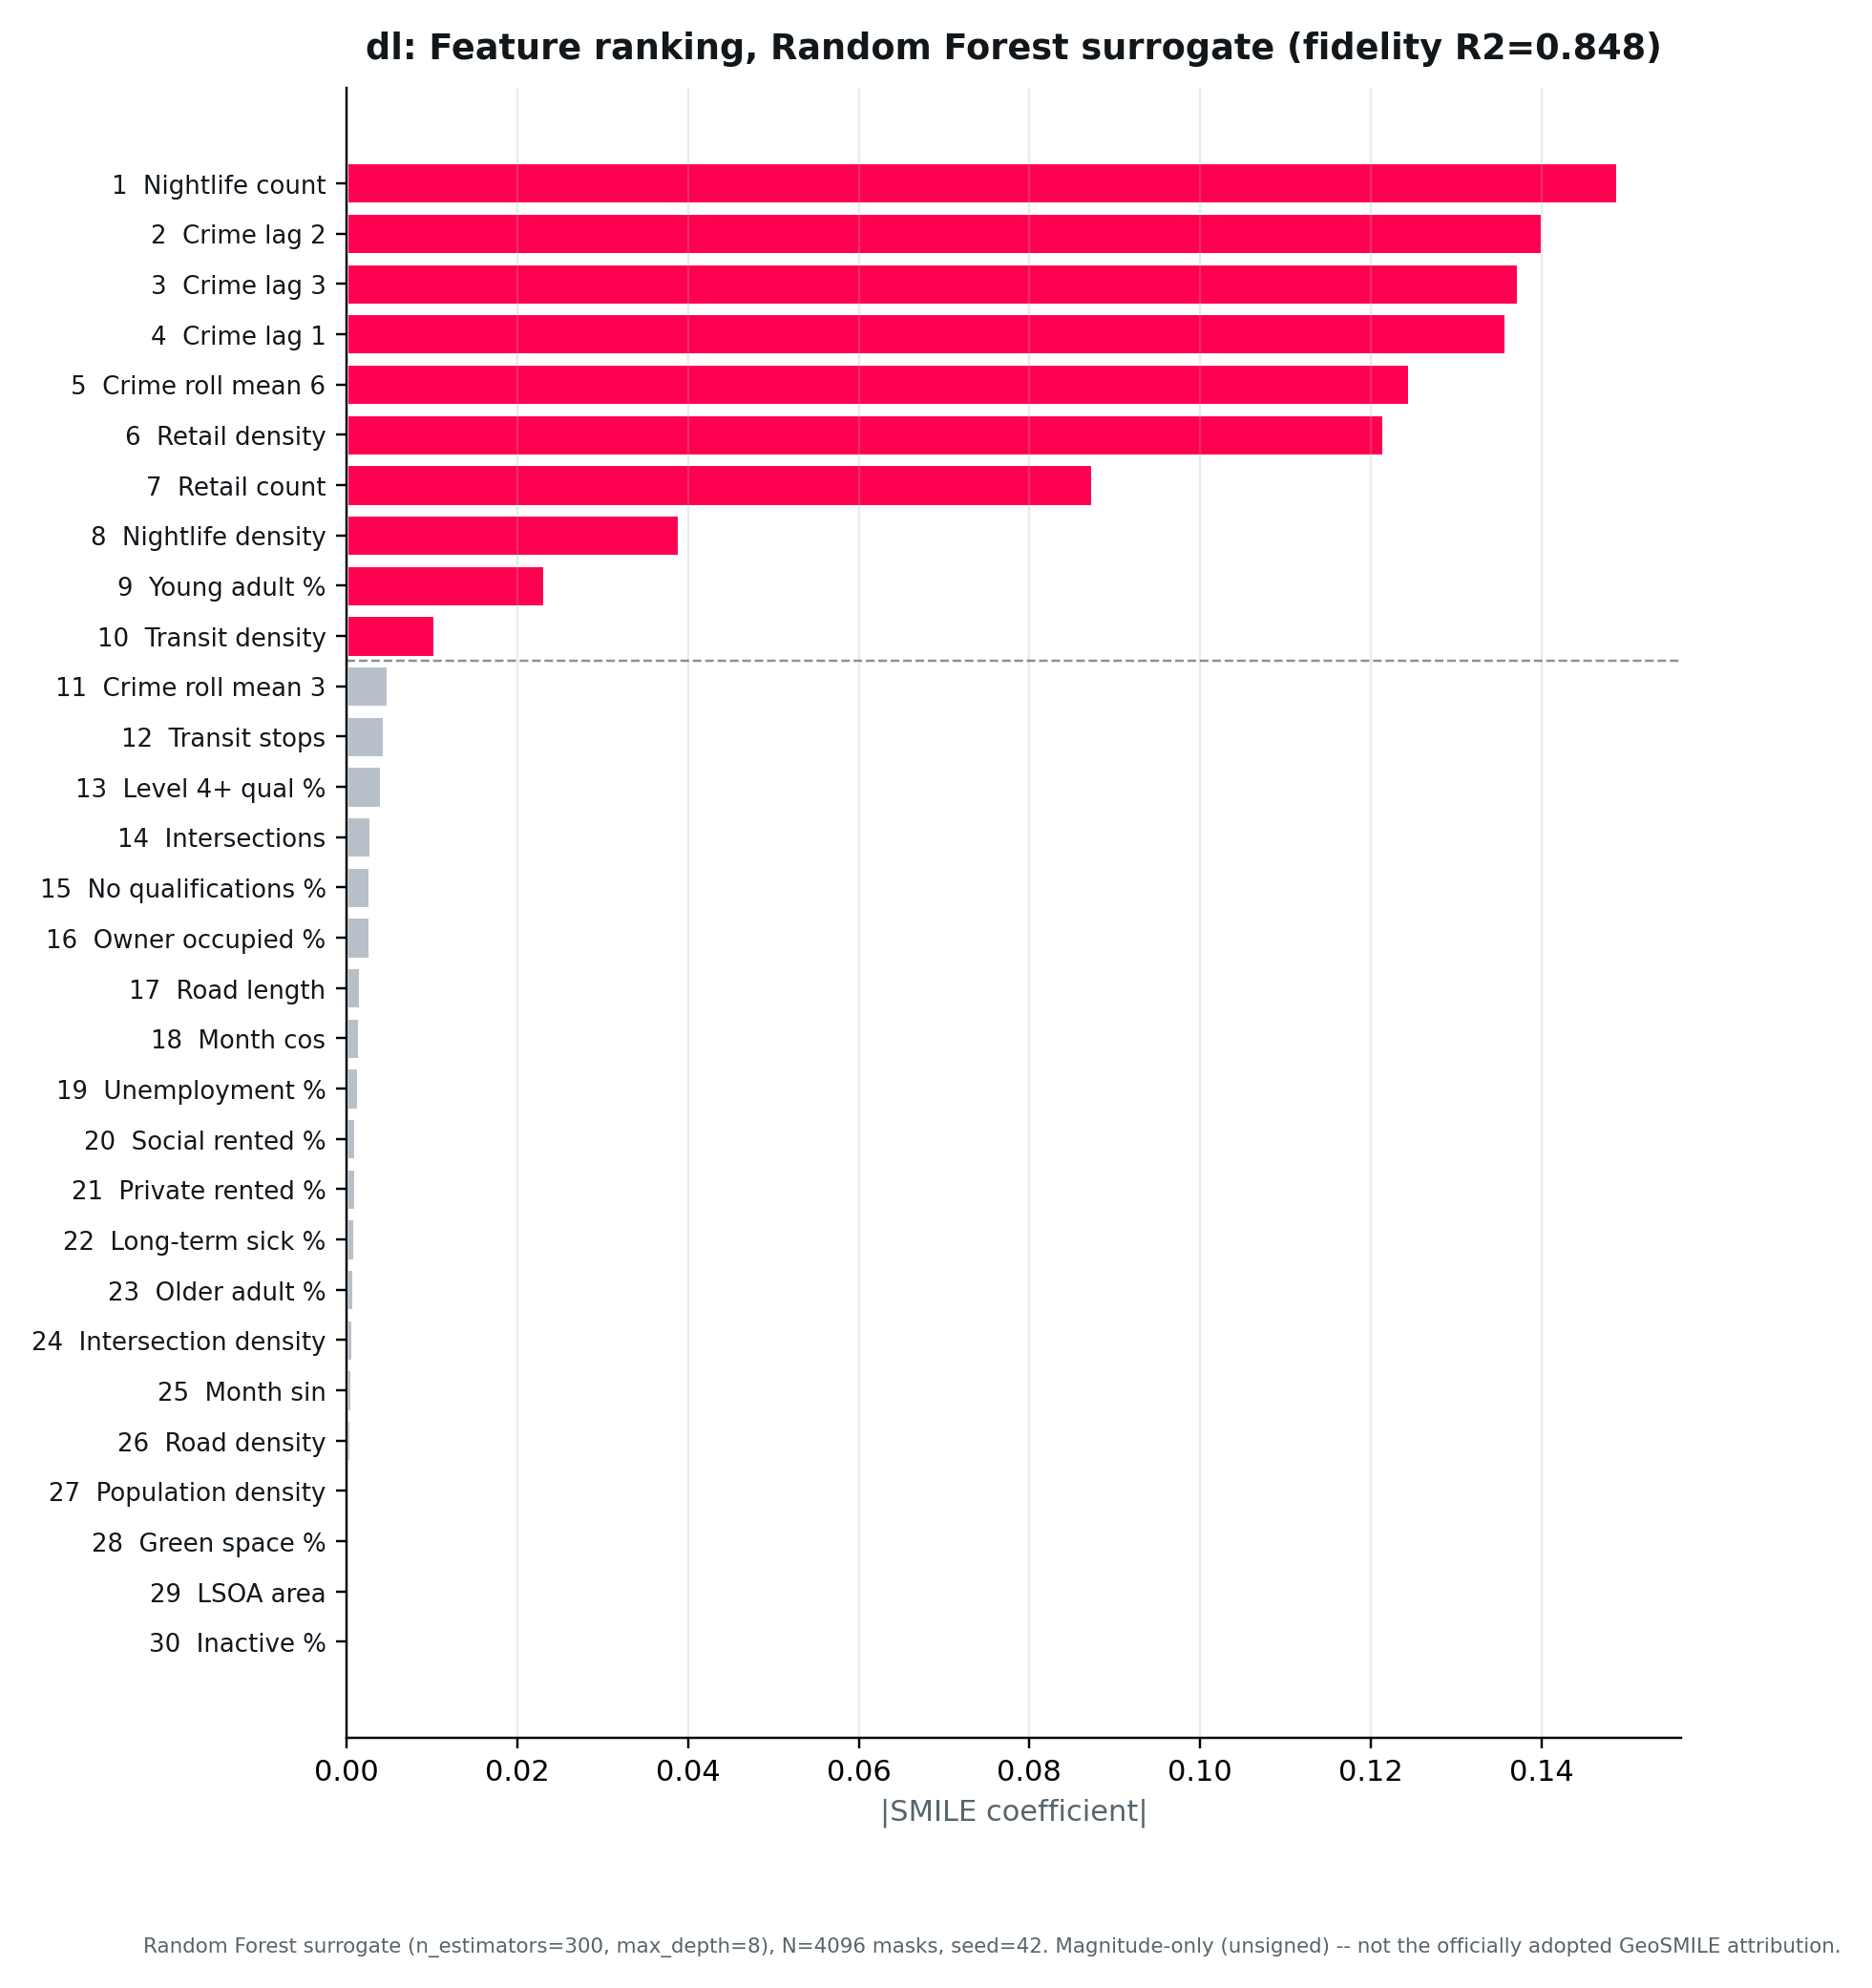
\includegraphics[width=\textwidth]{feature_top10_dl.png}
    \subcaption{DL (Keras)$^{\P}$ \\ {\scriptsize Random Forest, $N{=}4{,}096$, unweighted}}
    \label{fig:sel_feature_dl}
  \end{subfigure}
\caption{Feature ranking for the two models whose kernel-weighted Ridge
surrogate collapses (fidelity $R^2<0.13$, see
Table~\ref{tab:sel_provenance}) -- Random Forest \texttt{feature\_
importances\_} instead, magnitude-only (unsigned) and \emph{not} the
officially adopted GeoSMILE attribution (tree ensembles have no
linear-coefficient equivalent). Title reports \emph{fidelity} $R^2$, not
predictive $R^2$ -- the opposite of Figure~\ref{fig:sel_feature_ridge} --
because predictive fit was never the problem for either model (both exceed
$R^2=0.85$ predictively); it is the surrogate's ability to reconstruct the
masking response that this figure reports instead. Budget and weighting
also differ between the two panels below, each being that model's
best-found configuration in the surrogate$\times N$ sweep. Superscript
$\P$ marks this distinct provenance tier.}
\label{fig:sel_feature_rf}
\end{figure}
